\documentclass[a4paper]{article}
\input{../preamble.tex}
\newcommand{\lablsection}[1]{\section{#1}}
\newcommand{\lablsubsection}[1]{\subsection{#1}}
\newcommand{\assi}[6]{
	\draw[->] (#1,0) -- (#2,0) node[below]{$ #3 $};
	\draw[->] (0,#4) -- (0,#5) node[left]{$ #6 $};
	\draw (0,0) node[below left]{$ 0 $};
}
\newcommand{\assistd}[4]{\assi{-0.5}{#1}{#2}{-0.5}{#3}{#4}}
% \usepackage[acronym]{glossaries-extra}
% \setabbreviationstyle[acronym]{long-short}
% \newacronym{tvf}{TVF}{Teorema del valore finale}
% \newacronym{tvi}{TVI}{Teorema del valore iniziale}
% \newacronym{as}{A.S.}{Asintoticamente Stabile}
% \newacronym{fdt}{FdT}{Funzione di Trasferimento}
% \newacronym{siso}{SISO}{Single Input Single Output}
% \newacronym{mimo}{MIMO}{Multiple Input Multiple Output}
% \newacronym{lti}{LTI}{Lineari tempo invarianti}
% \newacronym{rh}{R-H}{Routh-Hurwitz}
% \makenoidxglossaries
\newcommand{\nota}[1]{\begin{figure}[H]\centering \Large$ \textcolor{gray}{\int} $\normalsize Nota: #1\end{figure}}
\newcommand{\person}[1]{\textsf{#1}}
\title{Fondamenti di Automatica}
\begin{document}
    \maketitle
    \tableofcontents
    % start lectures
    \lecture{1}{lun 01 mag 2023 16:51}{Intro}
	Iniziamo:
	\section{Definizioni}
	\begin{itemize}
		\item \textbf{Sistema}: cosa vogliamo controllare.
		\item \textbf{Controllo automatico}: senza o parziale controllo umano.
		\item \textbf{Controllo manuale}: azione esercitata dal l'operatore
	\end{itemize}
	\subsection{Notazione Standard}
	
	\begin{figure}[H]
		\begin{tikzpicture}[thick]
			\draw[->] (-9,0) -- (-8,0) node[above]{$ y^0 $} node[below,darkorange]{set point o riferimento}--(-7,0);
			\draw[rounded corners] (1,.5) rectangle (-1,-0.5); 
			\draw (0,0) node[scale=1.5]{S};
			\draw[->] (0,1.5) -- (0,1) node[above left]{d} -- (0,.5);
			\draw (0,1) node[above right,darkorange]{disturbo};
			\draw[->] (-3,0)node[below,darkorange]{variabile di controllo} --(-2,0)node[above]{u} -- (-1,0);
			\draw[<-] (3,0)node[below,darkorange]{variabile controllata} -- (2,0)node[above]{$ y $} -- (1,0);
			\draw (0,-.5) node[below,darkorange]{sistema};
		\end{tikzpicture}
		%		\centering
		%		\includegraphics[width=0.7\linewidth]{Images/notazione_standard}
		%		\caption{rappresentazione generica di un sistema}
		%		\label{fig:notazionestandard}
	\end{figure}
	Notazioni:
	\begin{itemize}
		\item \textbf{Disturbo}: Tutto quello che non so o tutto quello che agisce esternamente
		\item \textbf{Set Point}: Risultato che voglio raggiungere
		\item \textbf{Variabile manipolabile}: Cosa faccio per modificare il sistema
		\item \textbf{Controllata}: Risultato, Objective $y = y^0$
		\item \textbf{Problema di controllo}: Assegnare ad $u$ un valore tale che $ y= y^0 $ 
		\item \textbf{Legge di controllo}: criterio scelto per generare $ u $
	\end{itemize}
	\subsection{Sistema ad anello}
	\begin{figure}[H]
		\centering
		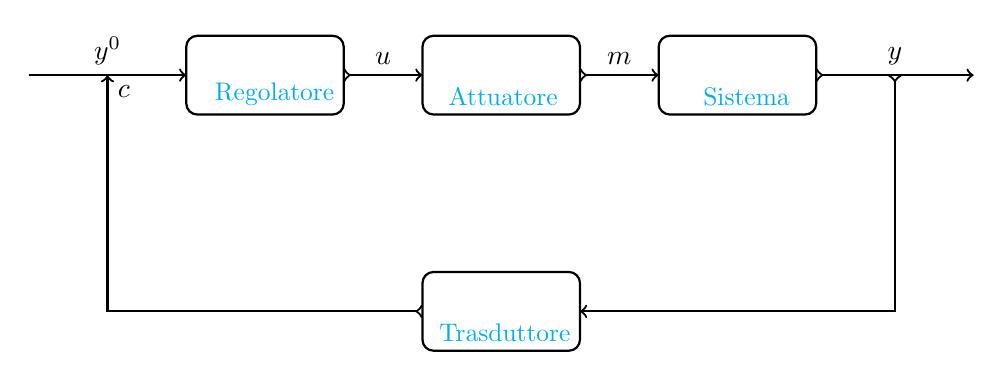
\begin{tikzpicture}[thick]
			\draw[->] (-5,0) -- (-4,0) node[above]{$ y^0 $} -- (-3,0);
			\draw[rounded corners] (-3,.5) rectangle (-1,-.5) node[above left, scale=0.92,cyan]{Regolatore};
			\draw[>->,xshift=3cm] (-4,0)--(-3.5,0) node[above]{$ u $} -- (-3,0);
			\draw[rounded corners,xshift=3cm] (-3,.5) rectangle (-1,-.5) node[above left, scale=0.92,cyan]{\, Attuatore \,};
			\draw[>->,xshift=6cm] (-4,0)--(-3.5,0) node[above]{$ m $} -- (-3,0);
			\draw[rounded corners,xshift=6cm] (-3,.5) rectangle (-1,-.5) node[above left, scale=0.92,cyan]{\,\, Sistema \,\,};
			\draw[>->,xshift=10cm] (-5,0)--(-4,0) node[above]{$ y $} -- (-3,0);
			\draw[>->] (6,0) -- (6,-3) -- (2,-3);
			\draw[rounded corners,xshift=3cm,yshift=-3cm] (-3,.5) rectangle (-1,-.5) node[above left, scale=0.92,cyan]{Trasduttore};
			\draw[<-<,rotate around y=180,xshift=2cm] (6,0)node[below right]{$ c $}  -- (6,-3) -- (2,-3);
		\end{tikzpicture}
		%		\includegraphics[width=0.7\linewidth]{"Images/Anello Chiuso"}
		\label{fig:anello-chiuso}
	\end{figure}
	
	Un sistema ad anello può essere suddiviso in due sotto-categorie: Anello \emph{Chiuso} e Anello \emph{Aperto}\\
	In figura è dato un sistema ad anello chiuso. In questo schema l'attuatore trasforma $ u $ in $ m $ (Esempio: voltaggio in energia meccanica $ \to $ Motore)


    \lecture{2}{lun 01 mag 2023 17:06}{Libreria di sistemi elementari}
	\lablsection{Libreria di sistemi elementari}
	% --- Resistore ---
	\lablsubsection{Resistore}
	\begin{figure}[H]
		\begin{minipage}{.3\textwidth}
			\centering
			\includegraphics[width=.4\linewidth]{"Images/resistore.png"}
		\end{minipage}%
		\begin{minipage}{.3\textwidth}
			\begin{itemize}
				\item R: resistenza
				\item V: tensione
				\item i: corrente
			\end{itemize}
		\end{minipage}
		\begin{minipage}{.3\textwidth}
			\centering
			\begin{equation*}
				\boxed{\text{V} = \text{R}i}
			\end{equation*}
		\end{minipage}
	\end{figure}
	
	% --- Induttore ---
	\lablsubsection{Induttore}
	\begin{figure}[H]
		\begin{minipage}{.3\textwidth}
			\centering
			\includegraphics[width=.4\linewidth]{"Images/induttore.png"}
		\end{minipage}%
		\begin{minipage}{.3\textwidth}
			\begin{itemize}
				\item L: induttanza
				\item V: tensione
				\item i: corrente
			\end{itemize}
		\end{minipage}
		\begin{minipage}{.3\textwidth}
			\centering
			\begin{equation*}
				\boxed{\text{V} = \text{L}\frac{di}{dt} = \text{L} \dot{i}}
			\end{equation*}
		\end{minipage}
	\end{figure}
	
	% --- Condensatore ---
	\lablsubsection{Condensatore}
	\begin{figure}[H]
		\begin{minipage}{.3\textwidth}
			\centering
			\includegraphics[width=.4\linewidth]{"Images/condensatore.png"}
		\end{minipage}%
		\begin{minipage}{.3\textwidth}
			\begin{itemize}
				\item C: capacità
				\item V: tensione
				\item i: corrente
			\end{itemize}
		\end{minipage}
		\begin{minipage}{.3\textwidth}
			\centering
			\begin{equation*}
				\boxed{\frac{d\text{V}}{dt} = \frac{1}{\text{C}}i}
			\end{equation*}
		\end{minipage}
	\end{figure}
	
	% --- Massa ---
	\lablsubsection{Massa}
	\begin{figure}[H]
		\begin{minipage}{.3\textwidth}
			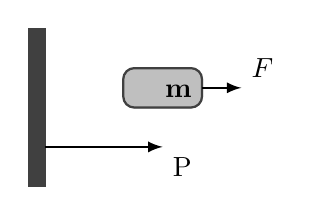
\begin{tikzpicture}[thick]
				\filldraw[color=darkgray] (-.2,0) rectangle (0,2);
				\draw[-latex] (0,.5) -- (1.5,.5)node[below right]{P};
				\filldraw[rounded corners,lightgray] (1,1.5) rectangle (2,1) node[above left,black]{$ \textbf{m} $};
				\draw[rounded corners,darkgray] (1,1.5) rectangle (2,1);
				\draw [-latex] (2,1.25) -- (2.5,1.25) node[above right]{$ F $};
			\end{tikzpicture}
			%			\includegraphics[width=.6\linewidth]{"Images/massa.png"}
		\end{minipage}%
		\begin{minipage}{.3\textwidth}
			\begin{itemize}
				\item M: massa
				\item P: posizione
				\item v: velocità
				\item a: accelerazione
				\item F: forza
			\end{itemize}
		\end{minipage}
		\begin{minipage}{.3\textwidth}
			\centering
			\begin{equation*}
				\boxed{F = ma}\text{  }
				\boxed{a = \frac{dv}{dt}}\text{  }
				\boxed{v = \frac{dP}{dt}}
			\end{equation*}
		\end{minipage}
	\end{figure}
	
	% --- Oscillatore Armonico ---
	\lablsubsection{Oscillatore armonico}
	\begin{figure}[H]
		\begin{minipage}{.3\textwidth}
			\includegraphics[width=.6\linewidth]{"Images/oscillatorearmonico.png"}
			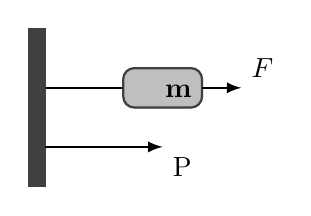
\begin{tikzpicture}[thick]
				\draw[decorate,decoration={coil,segment length=5pt,aspect=0.7,amplitude=4pt,pre=lineto,pre length=5mm,post=lineto,post length=5mm},thick] (0,1.25) -- (1,1.25);
				\filldraw[darkgray] (-.2,0) rectangle (0,2);
				\draw[-latex] (0,.5) -- (1.5,.5)node[below right]{P};
				\filldraw[rounded corners,lightgray] (1,1.5) rectangle (2,1) node[above left,black]{$ \textbf{m} $};
				\draw[rounded corners,darkgray] (1,1.5) rectangle (2,1);
				\draw [-latex] (2,1.25) -- (2.5,1.25) node[above right]{$ F $};
			\end{tikzpicture}
		\end{minipage}%
		\begin{minipage}{.3\textwidth}
			\begin{itemize}
				\item M: massa
				\item P: posizione
				\item v: velocità
				\item a: accelerazione
				\item F: forza
				\item K: costante elastica
				\item $ \sigma $: coefficiente di attrito
			\end{itemize}
		\end{minipage}
		\begin{minipage}{.3\textwidth}
			\centering
			\begin{equation*}
				\boxed{F = Kp + \sigma v + Ma}
			\end{equation*}
		\end{minipage}
	\end{figure}
	
	% --- Pendolo Semplice ---
	\lablsubsection{Pendolo semplice}
	\begin{figure}[H]
		\begin{minipage}{.3\textwidth}
			\includegraphics[width=.6\linewidth]{"Images/pendolosemplice.png"}
		\end{minipage}%
		\begin{minipage}{.3\textwidth}
			\begin{itemize}
				\item M: massa
				\item $ \tau $: coppia
				\item $ \theta $: posizione angolare
				\item $ \omega $: velocità angolare
				\item $ \alpha $:accelerazione angolare
				\item $ l $: lunghezza
				\item $ g $: accelerazione gravitazionale
			\end{itemize}
		\end{minipage}
		\begin{minipage}{.3\textwidth}
			\centering
			\begin{equation*}
				\boxed{\alpha = \frac{d\omega}{dt}}\text{ }
				\boxed{\omega = \frac{d\theta}{dt}}\text{  }
				\tau = \underbrace{Ml^2\alpha + Mgl\sin\theta}_{\textit{non lineare}}
			\end{equation*}
		\end{minipage}
	\end{figure}
	
	% --- Serbatoio Cilindrico ---
	\lablsubsection{Serbatoio cilindrico}
	\begin{figure}[H]
		\begin{minipage}{.3\textwidth}
			\includegraphics[width=.6\linewidth]{"Images/serbatoiocilindrico.png"}
		\end{minipage}%
		\begin{minipage}{.3\textwidth}
			\begin{itemize}
				\item $ A_s $: area sezione
				\item $ h $: livello liquido
				\item $ q_i $: portata ingresso
			\end{itemize}
		\end{minipage}
		\begin{minipage}{.3\textwidth}
			\centering
			\begin{equation*}
				\boxed{q_i = A_s \dfrac{dh}{di}}
			\end{equation*}
		\end{minipage}
	\end{figure}
	
	%--- Serbatoio con Valvola ---
	\lablsubsection{Serbatoio con valvola}
	\begin{figure}[H]
		\begin{minipage}{.3\textwidth}
			\centering
			\includegraphics[width=0.9\linewidth]{"Images/serbatoioconvalvola.png"}
		\end{minipage}%
		\begin{minipage}{.3\textwidth}
			\begin{itemize}
				\item $ A_s $: area sezione
				\item $ h $: livello liquido
				\item $ q_i $: portata ingresso
				\item $ A_v $: area valvola
				\item $ k $: costante della valvola
			\end{itemize}
		\end{minipage}
		\begin{minipage}{.3\textwidth}
			\centering
			\begin{equation*}
				\boxed{q_u = \frac{dh}{dt}A_s}\text{  }q_i = \underbrace{A_s \dfrac{dh}{di} + k A_v \sqrt{h}}_{\textit{non lineare}}
			\end{equation*}
		\end{minipage}
	\end{figure}
%%% Local Variables:
%%% mode: latex
%%% TeX-master: "master"
%%% End:

    \lecture{3}{lun 01 mag 2023 17:10}{Sistema dinamico e moti}
	\lablsection{Sistema dinamico}
	\begin{figure}[H]
		\centering
			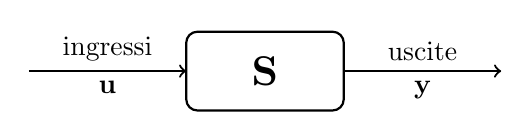
\begin{tikzpicture}[thick]
				\draw[<-] (3,0) -- (2,0)node[below]{$ \textbf{y} $} node[above]{uscite}-- (1,0);
				\draw[rounded corners] (1,.5) rectangle (-1,-0.5); 
				\draw (0,0) node[scale=1.5]{\textbf{S}};
				\draw[->] (-3,0) --(-2,0)node[below]{$ \textbf{u} $}node[above]{ingressi} -- (-1,0);
			\end{tikzpicture}
                        \end{figure}
			%			\includegraphics[width=0.9\linewidth]{"Images/sistemadinamico.png"}
			Ingresso: influenza il sistema\\
			Uscita: obiettivo del problema: vogliamo che tenda ad un riferimento ($ y^0 $)\\
	\nota{La relazione tra $ u $ e $ y $ è di causa effetto.}
	\begin{itemize}
		\item Occorre conoscere le equazioni differenziali
		\item Per risolverlo ci servono gli ingressi istante per istante
		\item Servono le condizioni iniziali
	\end{itemize}
	\lablsubsection{Ordine del sistema}
	Il numero di condizioni iniziali per determinare le uscite, noti gli ingressi istante per istante, è detto \emph{ordine del sistema} $ n $.
	\lablsubsection{Variabili di stato}
	Le $ n $ \emph{variabili di stato} si indicano come:
	\begin{figure}[H]
		\begin{minipage}{.4\textwidth}
			\centering
			\begin{equation*}
				\boxed{x_1,x_2,\dots,x_n}
			\end{equation*}
		\end{minipage}
		\begin{minipage}{.4\textwidth}
			\centering
			\begin{itemize}
				\item $ n $: numero variabili di stato
				\item $ m $: numero ingressi
				\item $ p $: numero uscite
			\end{itemize}
		\end{minipage}
	\end{figure}
	
	\subsubsection{Sistema dinamico in spazio di stato}
	\begin{align*}
		\dot{x}_1 &= f_1(x_1,x_2,\dots,x_n,u_1,u_2,\dots,u_m)\\
		\vdots &\\
		\dot x_n &= f_n(x_1,x_2,\dots,x_n,u_1,u_2,\dots,u_m)
	\end{align*}
	
	\subsubsection{Trasformazione uscita}
	\begin{align*}
		\dot y_1 &= g_1(x_1,x_2,\dots,x_n,u_1,u_2,\dots,u_m)\\
		\vdots &\\
		\dot y_p &= g_p(x_1,x_2,\dots,x_n,u_1,u_2,\dots,u_m)
	\end{align*}
	\lablsubsection{Notazione vettoriale}
	\begin{figure}[H]
		\centering
		\begin{minipage}{0.3\textwidth}
			\centering
			$\underline{x}(t) = \begin{pmatrix} 	x_1 \\ \dots \\	x_n	\end{pmatrix}$
		\end{minipage}
		\begin{minipage}{0.3\textwidth}
			\centering
			$\underline{y}(t) = \begin{pmatrix} 	y_1 \\ \dots \\	y_p	\end{pmatrix}$
		\end{minipage}
		\begin{minipage}{0.3\textwidth}
			\centering
			$\underline{u}(t) = \begin{pmatrix}u_1 \\ \dots \\ u_m\end{pmatrix}$
		\end{minipage}
	\end{figure}
	\begin{figure}[H]
		\centering
		\begin{minipage}{0.4\textwidth}
			\centering
			$f(\underline{x},\underline{u}) = \begin{pmatrix} 	f_1(\underline{x},\underline{u}) \\ \dots \\ f_n(\underline{x},\underline{u})	\end{pmatrix}$
		\end{minipage}
		\begin{minipage}{0.4\textwidth}
			\centering
			$g(\underline{x},\underline{u}) = \begin{pmatrix} 	g_1(\underline{x},\underline{u}) \\ \dots \\ g_p()\underline{x},\underline{u}	\end{pmatrix}$
		\end{minipage}
	\end{figure}
	con $ \vec{x} \in \R^n $, $ \vec{y} \in \R^p $, $ \vec{u} \in \R^m $, $ f \in \R^{n\times m} $ e $ g \in\R^{n\times m} $.\\
	Osservazione: I sistemi considerati sono \emph{tempo-invarianti}, la scelta dell'asse temporale è fatta ponendo $ t_0 =  0$
	\lablsubsection{Classificazione dei sistemi}
	\begin{itemize}
		\item Sistemi \emph{lineari} o \emph{non lineari}
		\item Sistemi "\emph{SISO}" (Single-Input-Single-Output) con $ n = p = 1 $ oppure "\emph{MIMO}" (Multi-Input-Multi-Output)
		\item Sistemi \emph{strettamente propri} (quando $ g $ non dipende da $ u $) e \emph{propri} (quando $ g $ invece dipende da $ u $)
	\end{itemize}
	\subsubsection{Esempi di sistemi in spazio di stato}
	\begin{itemize}
		\item \textbf{Resistore}: $ y = i $, $ u = \text{V} $ $ \to y = \frac{1}{R}u $
		\item \textbf{Induttore}: $ x_1 = 1, u = \text{V}, y = x_1 \to \begin{cases}
			\dot{x}_1 = \frac{1}{L} u \\
			y = x_1
		\end{cases}$
		\item \textbf{Massa}: $ x_1 = p, x_2 = \text{V}, u = \text{F} \to \begin{cases}
			\dot{x}_1 = x_2\\
			\dot{x}_1 = \frac{1}{M}u\\
			y = x_1
		\end{cases}$	
		\item \textbf{Oscillatore armonico}: $ x_1 = p, x_2=\omega, u = \tau\to\begin{cases}
			\dot{x}_1=x_2\\
			\dot{x}_1 = \frac{1}{M}(-Kx_1-\sigma x_2 + u)\\
			y = x_1
		\end{cases} $
		
		\item \textbf{Pendolo}: $ x_1 =h,y=x_1,u=q_i \to\begin{cases}
			\dot{x}_1 = x_2\\
			\dot{x}_1 = -\frac{g}{l} \sin(x_1) + \frac{1}{Ml^2} u\\
			y = x_1
		\end{cases}$
		
		\item \textbf{Serbatoio con valvola}: $ x_1 = h, y = x_1,u=q_1\to \begin{cases}
			\dot{x}_1 = \frac{1}{A_s}u - k\frac{A_v}{A_s}\sqrt{x_1}\\
			y = x_1
		\end{cases} $
	\end{itemize}
	I sistemi si distinguono in non lineari e lineari.
	\lablsubsection{Sistemi lineari}
	I sistemi lineari sono composto dalle \emph{equazioni di stato} che possono essere generalizzate come segue:
	\begin{equation*}
		\begin{cases}
			\dot{x}_1 = a_{11}x_1+a_{12}x_2+\dots+a_{1n}x_n+b_{11}u_1 + \dots+b_{1m}u_m\\
			\dots\\
			\dot{x}_n = a_{n1}x_1+a_{n2}x_2+\dots+a_{nn}x_n+b_{n1}u_1 + \dots+b_{nm}u_m\\
		\end{cases}
	\end{equation*}
	dalle trasformazioni di uscita:
	\begin{equation*}
		\begin{cases}
			y_1 = c_{11}x_1+c_{12}x_2+\dots+c_{1n}x_n+d_{11}u_1 + \dots+d_{1m}u_m\\
			\dots\\
			y_p = c_{p1}x_1+c_{p2}x_2+\dots+c_{pn}x_n+d_{p1}u_1 + \dots+d_{pm}u_m\\
		\end{cases}
	\end{equation*}
	Posso ridurre i due sistemi di equazioni lineari usando quattro matrici:
	\begin{figure}[H]
		\centering
		\begin{minipage}{.5\textwidth}
			\centering
			\[
			A = \begin{bmatrix}
				a_{11} & a_{12} & a_{13} & \dots & a_{1n} \\
				a_{21} & a_{22} & a_{23} & \dots & a_{2n} \\
				\vdots & \vdots & \vdots & \ddots & \vdots \\
				a_{n1} & a_{n2} & a_{n3} & \dots & a_{nn}
			\end{bmatrix}
			\]
		\end{minipage}%
		\begin{minipage}{.5\textwidth}
			\centering
			\[
			B = \begin{bmatrix}
				b_{11} & b_{12} & b_{13} & \dots & b_{1m} \\
				b_{21} & b_{22} & b_{23} & \dots & b_{2m} \\
				\vdots & \vdots & \vdots & \ddots & \vdots \\
				b_{n1} & b_{n2} & b_{n3} & \dots & b_{nm}
			\end{bmatrix}
			\]
		\end{minipage}
		
		\vspace{.1cm}
		
		\begin{minipage}{.5\textwidth}
			\centering
			\[
			C = \begin{bmatrix}
				c_{11} & c_{12} & c_{13} & \dots & c_{1p} \\
				c_{21} & c_{22} & c_{23} & \dots & c_{2p} \\
				\vdots & \vdots & \vdots & \ddots & \vdots \\
				c_{n1} & c_{n2} & c_{n3} & \dots & c_{np}
			\end{bmatrix}
			\]
		\end{minipage}%
		\begin{minipage}{.5\textwidth}
			\centering
			\[
			D = \begin{bmatrix}
				d_{11} & d_{12} & d_{13} & \dots & d_{1m} \\
				d_{21} & d_{22} & d_{23} & \dots & d_{2m} \\
				\vdots & \vdots & \vdots & \ddots & \vdots \\
				d_{n1} & d_{n2} & d_{n3} & \dots & d_{nm}
			\end{bmatrix}
			\]
		\end{minipage}
	\end{figure}
	Dunque il problema può essere riassunto nel seguente sistema:
	\begin{equation*}
		\begin{cases}
			\underline{\dot{x}} = \hat{A}\underline{x}+ \hat{B}\underline{u}\\
			\underline{y} = \hat{C}\underline{x}+\hat{D}\underline{u}
		\end{cases}
	\end{equation*}
	\lablsubsection{Movimento (moto)}
	Il moto dello stato è l'evoluzione nel tempo del vettore di stato date le condizioni iniziali e gli andamenti degli ingressi. Analoga è la definizione di moto dell'uscita. In generale, le equazioni del moto dello stato sono utilizzate per descrivere come i segnali di ingresso influenzano lo stato del sistema e come lo stato del sistema cambia nel tempo. Possono anche essere utilizzate per calcolare le risposte del sistema a determinate perturbazioni o a segnali di ingresso specifici.\\
	Per i sistemi lineari distinguiamo due termini di moto:
	\begin{enumerate}
		\item \textbf{Moto libero}: dipende dalle condizioni iniziali
		\item \textbf{Moto forzato}: dipende dagli ingressi
	\end{enumerate}
	In generale il moto è la somma di una componente libera e di una forzata.
	\begin{figure}[H]
		\begin{minipage}[t]{0.5\textwidth}
			\subsubsection{Moto libero}
			\begin{align*}
				x_l(t) = &e^{at}x_0\\
				y_l(t) = C&e^{at}x_0
			\end{align*}
		\end{minipage}
		\begin{minipage}[t]{0.5\textwidth}
			\subsubsection{Moto forzato}
			\begin{align*}
				x_f(t) = &\int^t_0 e^{a(t-\tau)}bu(\tau)\,d\tau\\
				y_f(t) =C&\int^t_0 e^{a(t-\tau)}bu(\tau)\,d\tau
			\end{align*}
		\end{minipage}
	\end{figure}
	
	\lablsubsection{Equilibri (moti costanti)}
	Supponiamo che  $u = \overline{u}$ , $\overline{u}$ costante.\\
	L'equilibrio corrispondente a $\overline{u}$ è il moto  costante di stato e uscita. Andando a sostituire nelle varie equazioni possiamo dedurre che:
	\[    \dot{x} = 0 \]
	\[\dot{x} = f(x,u) \to f(\overline{x},\overline{u} = 0\]
	\[\overline{x} : \text{Stati di equilibrio}\]
	\[\overline{y} = g(\overline{x},\overline{u})\]

%%% Local Variables:
%%% mode: latex
%%% TeX-master: "master"
%%% End:

    \lecture{4}{lun 01 mag 2023 17:12}{Sovrapposizione degli effetti, variabili di stato}
	\lablsection{Principio di sovrapposizione degli effetti}
	Vale per i sistemi lineari. Consideriamo tre casi:\\
	\begin{enumerate}
		\item $ \dot{x}_0 $ condizione iniziale, $ \dot{u}(t) $ per $ t \geq 0 $, ingresso $ \dot{x}(t), \dot{y}(t) $ moti di stato e uscita.
		\item $ \ddot{x}_0 $ condizione iniziale, $ \ddot{u}(t) $ per $ t \geq 0$ ingresso $ \ddot{x}(t), \ddot{y}(t) $ moti di stato e uscita.
		\item $ \dddot{x}_0=\alpha\dot{x}_0 +\beta\ddot{x}_0 $ condizione iniziale, $ \dddot{u}(t) $ per $ t \geq 0$ ingresso,$ \ddot{u}(t) = \alpha\dot{u}+\beta\ddot{u} $, $ \dddot{x}(t), \dddot{y}(t) $ moti di stato e uscita
	\end{enumerate}
	Il principio di sovrapposizione degli effetti dice che:\\
	\begin{align*}
		\dddot{x}(t) &= \alpha\dot{x} + \beta\ddot{x}\\
		\dddot{y}(t) &= \alpha\dot{y} + \beta\ddot{y}
	\end{align*}
	\lablsubsection{Matrice esponenziale}
	\begin{figure}[H]
		\begin{minipage}{0.5\textwidth}
			\begin{align*}
				\dot x &= Ax+Bu\\
				y &= Cx + Du
			\end{align*}
		\end{minipage}
		\begin{minipage}{0.5\textwidth}
			\centering
			\[A \in \R^{n\times n} \to\text{Quadrata}\] Si dice matrice della \emph{dinamica}
			\[ t\geq 0  \] 
		\end{minipage}
	\end{figure}
	\subsubsection{Definizione matrice esponenziale}
	\begin{equation*}
		\boxed{e^{\text At} = \sum_{k = 0}^{\infty}\frac{(\text At)^k}{k!} = I + \text At + \frac{\text A^2t^2}{2!}+\dots}
	\end{equation*}
	\\
	Si tenga in considerazione che la derivata della matrice esponenziale è calcolabile come segue:\\
	\begin{equation*}
		\frac{de^{\text{A}t}}{dt}  = \text Ae^{\text{A} t} = 0 + \text{A} + \frac{2\text A^2 t^2}{2!} + \dots
	\end{equation*}
	\nota{la matrice esponenziale può essere sorta per una generica $ \text{A} $. Noi consideriamo le matrici diagonalizzabili, cioè che $ \exists T | \det(t) \neq 0 $:
		\begin{equation*}
			\hat{A} = TAT^{-1} = diag(\lambda_1 \,\, \lambda_2 \,\,\dots\,\,\lambda_n)
	\end{equation*}}
	\lablsubsection{Formule di Lagrange}
	\begin{align*}
		x(t) &= e^{\text{A}(t-t_0)} x_0+ \int_{t_0}^{t}e^{\text{A}t-\tau}Bu(\tau)d\tau\\
		y(t) &= Ce^{\text{A}(t-t_0)}x_0+ C \int_{t_0}^{t}e^{\text{A}t-\tau}Bu(\tau)d\tau
	\end{align*}
	Sono le soluzioni di:
	\begin{align*}
		\begin{cases}
			\dot{x} =Ax+Bu\\
			y = Cx+Du
		\end{cases}
	\end{align*}
	\lablsubsection{Cambiamento delle variabili di stato}
	\begin{equation*}
		\begin{cases}
			\dot{x}(t) &=Ax(t)+Bu(t)\qquad(1)\\
			y(t) &= Cx(t)+Du(t)\qquad(2)
		\end{cases}
	\end{equation*}
	La scelta iniziale dello stato è il vettore $ x  = [x_1 \,\,\dots\,\,x_n]^T$. Voglio trovare la relazione $ T $ tra $ x $ e una nuova scelta del vettore di stato $ \hat{x} $ con $ \det(T)\neq0 $. \\
	$ \hat{x} $ è tale che:
	\begin{equation*}
		\boxed{\hat{x} = Tx}
	\end{equation*}
	\begin{equation*}
		\boxed{x = T^{-1}\hat{x}}
	\end{equation*}
	Eseguiamo delle sostituzioni nell'equazione (1) e moltiplico per $ T $:
	\[
	T\dot{x} = \text{TAT}^{-1}\hat{x}+\text{TB}u
	\]
	\[
	\boxed{\dot{\hat{x}} = \text{TAT}^{-1}\hat{x}+\text{TB}u}
	\]
	Faccio le sostituzioni in (2)
	\[y = CT^{-1}\hat{x}+ Du\]
	Chiamo:
	\begin{align*}
		\hat{A} = TAT^{-1}& \qquad &\hat{B} = TB\\
		\hat{C} = CT^{-1}& \qquad &\hat{D} = \hat{D}
	\end{align*}
	Trovo un sistema equivalente:
	\begin{equation*}
		\begin{cases*}
			\dot{\hat{x}} = \hat{A}\hat{x}+\hat{B}u\\
			y = \hat{C}\hat{x} + \hat{D}u
		\end{cases*}
	\end{equation*}
	\lablsubsection{Proprietà strutturale}
	Qualsiasi proprietà indipendente dalla scelta delle variabili di stato, quindi della matrice $ \text T $, è detta \emph{strutturale}.


%%% Local Variables:
%%% mode: latex
%%% TeX-master: "master"
%%% End:

    \lecture{5}{lun 01 mag 2023 17:12}{Stabilità}
	\lablsection{Stabilità}
        \twomini{
		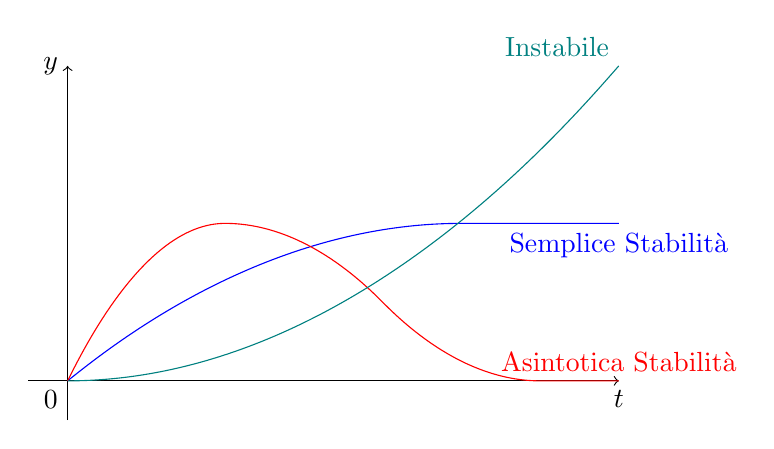
\begin{tikzpicture}
			\assistd{7}{t}{4}{y}
			\draw[color=blue] (0,0) parabola[bend at end] (5,2)--(7,2)  node[below] {Semplice Stabilità};
			\draw[color=red] (0,0) parabola bend (2,2)(4,1) parabola bend(6,0) (6,0) -- (7,0) node[above] {Asintotica Stabilità};
			\draw[color=teal] (0,0) parabola (7,4) node[above left] {Instabile};
		\end{tikzpicture}
}{	
	%\begin{figure}[H]
	%	\centering
	%	\includegraphics[width=0.7\linewidth]{Images/stabilità}
	%	\caption{Grafico dell'uscita rispetto al tempo con analisi sulla stabilità}
	%	\label{fig:stabilita}
	%\end{figure}
	Valutiamo il comportamento di $ y $ a fronte di perturbazioni. Per fare questo:
	\begin{itemize}[label*=$ - $]
		\item Perturbo la condizione iniziale
		\item Uso le definizioni di Lyapunov
		\item Dato $ v\in\R^n $ $ ||V|| = \sqrt{V^2_1+ \dots +V^2_n} $
	\end{itemize}
	A questo punto, definisco:
	\begin{itemize}[]
		\item Nominale:\\ $ \ast $ $ x_{N_0} $: condizione iniziale nominale\\  $ \ast $ $ x_N(t) $: movimento corrispondente generato applicando $ u(t) $ $ t\geq0 $
		\item Perturbata:\\  $ \ast $ $ x_{P_{0}} $: condizione iniziale perturbata\\  $\ast$ $ x_P(t) $: movimento corrispondente generato applicando $ u(t) $ $ t\geq0 $
	\end{itemize}}
	\lablsubsection{Semplice stabilità del moto}
	Il moto $ x_N $(t) si dice \emph{stabile} se $ \forall\varepsilon>0 $ esiste $ \delta_\varepsilon>0 $ tale che $ \forall x_{P_{0}}$ per cui $ \vvline x_{P_0}-x_{N_0}\vvline \leq \delta_\varepsilon$ allora: 
	\begin{figure}[H]
		\begin{minipage}{0.5\textwidth}
			\begin{equation*}
				\vvline x_P(t) -x_N(t)\vvline\leq\varepsilon\qquad\forall t\geq0
			\end{equation*}
		\end{minipage}
		\begin{minipage}{0.5\textwidth}
			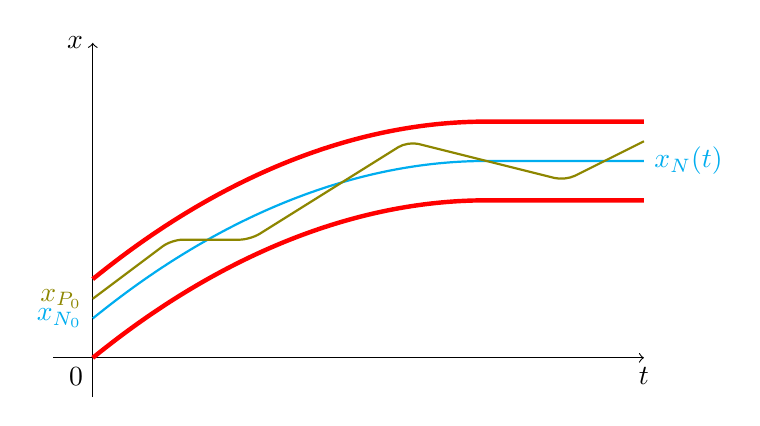
\begin{tikzpicture}
				\assistd{7}{t}{4}{x}
				\draw[ultra thick,color=red] (0,0) parabola[bend at end] (5,2)--(7,2);
				\draw[ultra thick,color=red] (0,1) parabola[bend at end] (5,3)--(7,3);
				\draw[color=cyan,thick] (0,.5)node[left]{$ x_{N_0} $} parabola[bend at end] (5,2.5)--(7,2.5) node[right]{$ x_N(t) $};
				\draw[color=olive,thick,rounded corners] (0,0.75)node[left]{$ x_{P_0} $} -- (1,1.5) -- (2,1.5)-- (4,2.75) -- (6,2.25) -- (7,2.75);
			\end{tikzpicture}
		\end{minipage}
	\end{figure}
	\lablsubsection{Asintotica stabilità del moto}
	Il moto $ x_N $(t) si dice \emph{Asintoticamente stabile} se  è stabile e:
	\begin{figure}[H]
		\begin{minipage}{0.5\textwidth}
			\begin{equation*}
				\Large\lim_{t\to+\infty}\vvline x_P(t) -x_N(t)\vvline=0
			\end{equation*}
			\[\forall x_{P_0}: \vvline x_P(t) -x_N(t)\vvline\leq\delta_\varepsilon\]
		\end{minipage}
		\begin{minipage}{0.5\textwidth}
			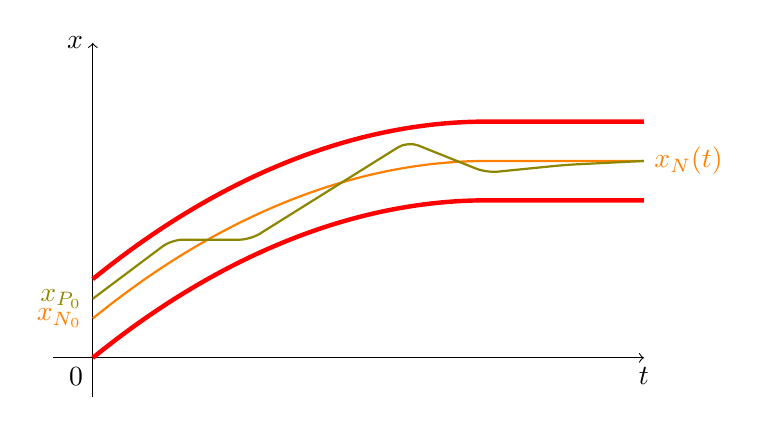
\begin{tikzpicture}
				\assistd{7}{t}{4}{x}
				\draw[ultra thick,color=red] (0,0) parabola[bend at end] (5,2)--(7,2);
				\draw[ultra thick,color=red] (0,1) parabola[bend at end] (5,3)--(7,3);
				\draw[color=orange,thick] (0,.5)node[left]{$ x_{N_0} $} parabola[bend at end] (5,2.5)--(7,2.5)node[right]{$ x_N(t) $};
				\draw[color=olive,thick,rounded corners] (0,0.75)node[left]{$ x_{P_0} $} -- (1,1.5) -- (2,1.5)-- (4,2.75) -- (5,2.35) -- (6,2.45) -- (7,2.5);
			\end{tikzpicture}
		\end{minipage}
	\end{figure}
	\lablsubsection{Instabilità del moto}
	\begin{figure}[H]
		\begin{minipage}{0.5\textwidth}
			Se non vale la condizione di stabilità, le traiettorie divergono e il moto si dice \emph{instabile}:
		\end{minipage}
		\begin{minipage}{0.5\textwidth}
			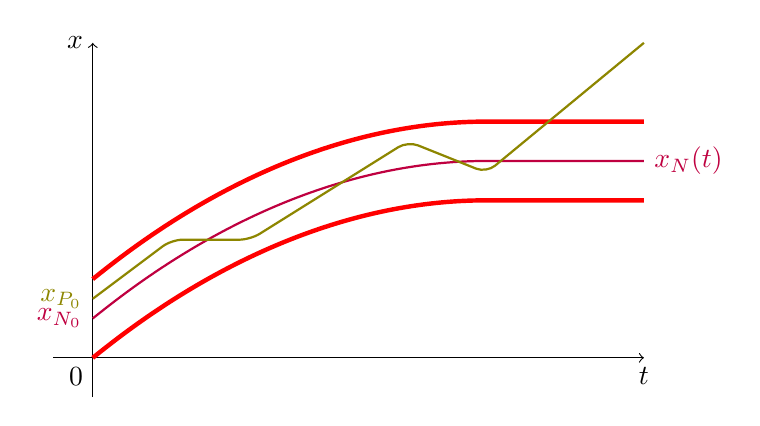
\begin{tikzpicture}
				\assistd{7}{t}{4}{x}
				\draw[ultra thick,color=red] (0,0) parabola[bend at end] (5,2)--(7,2);
				\draw[ultra thick,color=red] (0,1) parabola[bend at end] (5,3)--(7,3);
				\draw[color=purple,thick] (0,.5)node[left]{$ x_{N_0} $} parabola[bend at end] (5,2.5)--(7,2.5)node[right]{$ x_N(t) $};
				\draw[color=olive,thick,rounded corners] (0,0.75)node[left]{$ x_{P_0} $} -- (1,1.5) -- (2,1.5)-- (4,2.75) -- (5,2.35) -- (7,4);
			\end{tikzpicture}
		\end{minipage}
	\end{figure}
	Tutte le definizioni per ora scritte valgono anche per gli \emph{equilibri} (moti costanti), è sufficiente sostituire $ x_N(t) $ con $ \overline{x_N}\quad\forall t\geq0 $\\
	\nota{Gli equilibri possono soddisfare diverse definizioni di stabilità (vedi esempio seguente)}
	\begin{figure}[H]
		\centering
		\begin{minipage}{0.3\textwidth}
			\begin{tikzpicture}[font=\footnotesize]
				% Support
				\draw[pattern=dots] (0,0) circle(.25cm);
				\draw[->,color=purple] (0,-1) arc[start angle=-90,end angle=-60,radius=1];
				\draw[color=purple] (0.5,-0.75) node[right]{$ \tau = \vartheta $};
				\draw[color=darkgray] (0.25,0) node[above right]{Pendolo};
				\draw[dashed,color=gray] (0,0) -- (-90:4);
				% Rod + Bob
				\draw (0,0) -- (-60:4) node[fill,circle](m){};
				
				% Weight Force
				\draw[-latex] (m) -- node[right]{$\vec{Mg}$}++(0,-1) ;
			\end{tikzpicture}
			
		\end{minipage}
		\begin{minipage}{0.3\textwidth}
			\centering
			\begin{tikzpicture}[font=\footnotesize]
				% Support
				\draw[pattern=dots] (0,0) circle(.25cm);
				\draw[color=red] (-0.25,0) node[above left]{Instabile} node[below left,purple]{$ \tau = 180$° };
				\draw[->,color=purple] (0,-1) arc[start angle=-90,end angle =90,radius = 1];
				\draw[dashed,color=gray] (0,0) -- (-90:4);	
				% Rod + Bob
				\draw (0,0) -- (90:4) node[fill,circle](m){};
				
				% Weight Force
				\draw[-latex] (m) -- node[right]{$\vec{Mg}$}++(0,-1) ;
			\end{tikzpicture}
		\end{minipage}
		\begin{minipage}{0.3\textwidth}
			\centering
			\begin{tikzpicture}[font=\footnotesize]
				% Support
				\draw[pattern=dots] (0,0) circle(.25cm);
				\draw[color=green] (0.25,0) node[above right]{Stabile} node[below right]{$\tau =0$°};
				% Rod + Bob
				\draw (0,0) -- (-90:4) node[fill,circle](m){};
				
				% Weight Force
				\draw[-latex] (m) -- node[right]{$\vec{Mg}$}++(0,-1) ;
			\end{tikzpicture}
		\end{minipage}
	\end{figure}
	\lablsubsection{Regione di attrazione}
	Per gli stati \emph{Asintoticamente stabili} definiamo regione di attrazione l'insieme dei punti partendo dai quali si converge all'equilibrio.
	\begin{figure}[H]
		\centering
		\begin{tikzpicture}
			\newcommand{\var}{4}
			\assi{-\var}{\var}{x_1}{-\var}{\var-1}{x_2}
			\filldraw[color=darkpurple] (0,0) node[fill,circle](m){};
			\draw[color=darkpurple] (0,0) node[above right] {Equilibrio};
			\draw[color=red,rotate=45,thick] (2,1) -- (0,1) node[red,rotate=45,above,in front of path,scale=1.25] {Regione di attrazione} -- (-2,1) -- (-3,-2) -- (3,-2)--cycle;
		\end{tikzpicture}
	\end{figure}
	\nointerlineskip


%%% Local Variables:
%%% mode: latex
%%% TeX-master: "master"
%%% End:

    \lecture{6}{lun 01 mag 2023 17:13}{Criteri di Stabilità}
        \lablsection{Stabilità dei sistemi LTI}
	Per i sistemi non lineari \underline{non} ha senso parlare di stabilità del sistema in toto ma posso parlare di stabilità di alcuni moti.\\
	Per i sistemi \emph{LTI} invece si parla di stabilità del sistema. Come già detto in precedenza le definizioni di moti nominale e perturbati sono:
	\begin{equation*}
		\begin{cases*}
			\dot{x}_N(t) = Ax_N(t)+ Bu(t) \quad t \geq0 \quad x_{N_0} = x_N(0) \quad (1)\\
			\dot{x}_P(t) = Ax_P(t)+ Bu(t) \quad t \geq0 \quad x_{P_0} = x_P(0) \quad (2)
		\end{cases*}
	\end{equation*}
	Sottraendo (1) a (2):
	\begin{equation*}
		\dot{x}_P -\dot{x}_N = A(x_P-x_N)\quad x_{P_0}-x_{N_0} = x_P(0)-x_N(0) 
	\end{equation*}
	Chiamo:
	\[
	\delta x = x_P -x_N \quad\delta x_0 = X_{P_0} - x_{N_0}
	\]
	\[
	\boxed{	\delta \dot{x} = A\delta x}
	\]
	\begin{table}[H]
		\centering
		\begin{minipage}[t]{0.4\textwidth}
			\lablsubsection{Definizione Stabilità}
			$ x_N(t) $ è \emph{stabile} se $ \forall\varepsilon>0\,\, \exists \delta_\varepsilon>0$ \\tale che $ \forall\delta x_0 $ per cui:\[\vvline\delta x_0\vvline\leq\delta_\varepsilon\]
			Allora:\[\vvline\delta x(t)\vvline\leq\varepsilon\quad\forall t\geq 0\]
		\end{minipage}
		\vline
		\hspace{2ex}
		\begin{minipage}[t]{0.4\textwidth}
			\lablsubsection{Definizione A.S.}
			$ x_N(t) $ è \emph{Asintoticamente Stabile} se è stabile e:
			\[\lim_{t\to+\infty}\vvline\delta x\vvline = 0 \quad \forall\delta x_0 : \vvline\delta x_0 \vvline\leq\delta_\varepsilon\]
		\end{minipage}
		
	\end{table}
	Noto che la soluzioni di $ \delta\dot{x} = A\delta x $ è il moto libero, cioè dipende da $ e^{At} $ e dalle condizioni iniziali. L'osservazione vale per tutti i moti, quindi la stabilità è una proprietà del sistema (\cref*{subsec:Proprietà strutturale}).Inoltre le soluzioni sono scalate dalle condizioni iniziali. Il moto libero è infatti:\\
	\[\delta x_\ell = e^{\text{A}t}\underline{\delta x_0}\]
	\lablsubsection{Stabilità e autovalori}
	Partiamo, per i sistemi \emph{LTI}, dal moto libero:
	\[x_\ell = e^{\text{A}tx_0}\]
	Se consideriamo matrici diagonalizzabili, $ \exists T: \det(T) \not=0 $ tale che 
	\[\hat{A} = TAT^{-1} = diag\{\lambda_1, \lambda_2,\dots,\lambda_n\} \qquad \lambda_i \text{ Autovalori}\]
	A questo punto scrivo esplicitamente il moto libero
	\[x_\ell(t) e^{T^{-1}\hat{A}T}x_0 = T^{-1}\large\left[\begin{matrix}
		e^{\lambda_1t} & && 0\\
		& e^{\lambda_2t}&&  \\
		& & \ddots&\\
		0 & & & e^{\lambda_nt}
	\end{matrix}\large\right] T x_0\] 
	Le soluzioni sono combinazioni lineari degli esponenti $ e^{\lambda_it} ,i =1,\dots,n$ e si chiamano \emph{modi}. Noto che gli autovalori possono essere reali o complessi coniugati: $ \lambda_i =\alpha_i +\jmath\beta_i $. Noto che la matrice $ A $ è reale e la matrice esponenziale contiene solo numeri reali, cioè le parti immaginarie si elidono tramite i prodotti per $ T $ e $ T^-1 $. Otterremo:
	\begin{equation*}
		\boxed{e^{\alpha_it}\sin(\beta_it+\varphi_i)}\qquad i=1,\dots,n
	\end{equation*}
	\lablsubsection{Teorema di stabilità dei sistemi LTI}
	Considero un sistema con $ A $ diagonalizzabile il sistema è:\\
	A.S se e solo se tutti gli autovalori di $ A $ hanno parte reale strettamente negativa ($\Re(\lambda)<0$)\\
	Dimostrazione:\\
	se $ \alpha_i\leq0 \,\,\forall i $, con almeno un autovalore a parte reale nulla, tutti i moti sono limitati nel tempo, in particolare quelli associati ad autovalori con parte reale nulla sono o costanti ($ \beta_i = 0 $), o oscillano ($ \beta_i \not=0 $).\\
	\colorbox{gray!20}{Instabile se e solo se esiste almeno un autovalore a parte reale positiva}\\
	Dimostrazione:
	Se esiste almeno un autovalore con parte reale positiva, cioè $ \exists \jmath : \alpha_i>0 $, allora esiste almeno un esponenziale che diverge.\\
	Gli autovalori sono disposti nel piano complesso.\\
	Osservazioni:
	\begin{itemize}
		\item La stabilità è una proprietà strutturale.
		\item Il teorema esprime una condizione necessaria e sufficiente affinché $ A $ sia diagonalizzabile.
		\item Se la matrice $ A $ non è diagonalizzabile, posso scrivere la forma di \person{Jordan}.
		\item Se $ A $ non è diagonalizzabile e ci sono autovalori a parte reale nulla, il sistema è instabile se per almeno uno degli autovalori a parte reale nulla la molteplicità geometrica è minore di quella algebrica.
	\end{itemize}
	\lablsubsection{Criterio degli autovalori}
	Data una matrice A diagonalizzabile:\\
	\begin{itemize}
		\item A.S. $\iff \Re(\lambda_i)<0 \space i = 1,\dots,n$
		\item Semplicemente stabile $\iff \Re(\lambda_i)\leq 0 \space i=1,\dots,n$
		\item Instabilità: $\exists \jmath : \Re(\lambda_j)>0$
	\end{itemize}
	\lablsubsection{Criteri di ispezione di A}
	\begin{enumerate}
		\item Se la matrice A è diagonale o triangolare, gli autovalori sono sulla diagonale.
		\item $ Tr(A) = \sum_{i =1}^{n} \lambda_i =\sum_{i=1}^{n}\Re(\lambda_i)$\\
		se la traccia è positiva o nulla il sistema non è A.S.; se è positiva in particolare è instabile
		\item $\det(A) =\prodc_{i=1}^{n}\lambda_i$\\
		se il determinante è nullo il sistema non è A.S.
	\end{enumerate}
	\lablsubsection{Criterio del polinomio caratteristico}
	\[\boxed{X(\lambda) =\det(\lambda I-A)}\]
	Posso calcolare le radici di questo polinomio e poi usare uno dei seguenti criteri:
	\subsubsection{Criteri basati sui coefficienti del polinomio caratteristico}
	\begin{itemize}
		\item \textbf{Polinomi di grado $ n=2 $}\\
		Condizioni necessarie e sufficienti perché il sistema sia A.S. è che i coefficienti di $ X(\lambda) $ siano concordi in segno.
		\item \textbf{Polinomi di grado $ n>2 $}\\
		Condizione solo necessaria perché il sistema sia A.S. è che tutti i coefficienti di $ X(\lambda) $ siano concordi in segno
	\end{itemize}
	Nel caso di $ n>2 $ va applicato un altro criterio:
	\subsubsection{Criterio di \person{Routh}-\person{Hurwitz} (R-H)}
	\begin{enumerate}
		\item Scrivo $ X(\lambda) $ e verifico che sia ordinato come segue\\
		$ X(\lambda) = \varphi_0\lambda^n + \varphi_1\lambda^{n-1} + \dots + \varphi_n $
		\item Costruisco la tabella di R-H di $ n+1 $ righe\\
		\begin{table}[H]
			\centering
			\begin{tabular}{c c c c}
				$\varphi_0$ & $\varphi_2$ & $\varphi_4$ & \dots \\
				$\varphi_1$ & $\varphi_3$ & $\varphi_5$ & \dots \\
				$ h_1 $   & $ h_2 $     & $ h_3 $     & \dots \\
				$ k_1 $   & $ k_2 $     & $ k_3 $     & \dots \\
				$ \ell_1 $  & $ \ell_2 $  & $ \ell_3 $  & \dots \\
				\vdots    &             &             &       \\
				n+1   &             &             &
			\end{tabular}
		\end{table}
		\[ h_i = -\frac{1}{\varphi_1} \det\left[\begin{matrix}
			\varphi_0 & \varphi_{2i}\\
			\varphi_1 & \varphi_{2i +1}
		\end{matrix}\right]  \quad i = 1,\dots\]
		\[ k_i = -\frac{1}{h_1} \det\left[\begin{matrix}
			\varphi_1 & \varphi_{2i+1}\\
			h_1 & h_{i +1}
		\end{matrix}\right]  \quad i = 1,\dots\]
		\item Verifico che i coefficienti della prima colonna siano diversi da zero, cioè la tabella di R-H è \emph{ben definita}
		\item Applico il criterio di \person{Routh-Hurwitz}:\\
		Il sistema è A.S. se e solo se la tabella di R-H è ben definita e tutti gli elementi della prima colonna sono concordi in segno.
		\item Verifico che i coefficienti della prima colonna siano diversi da zero, cioè la tabella di R-H è "ben-definita".
		\item Applico il criterio di R-H:\\
		Il sistema è A.S se e solo se la tabella di R-H è ben definita e tutti gli elementi della prima colonna sono concordi in segno
	\end{enumerate}

    \input{lec_07.tex}
    \lecture{8}{lun 01 mag 2023 17:14}{Linearizzazione}
	\lablsection{Linearizzazione}
	Consideriamo piccoli spostamenti nell'interno dei punti di equilibrio. Considero un'approssimazione lineare nell' intorno del punto
	\begin{equation*}
		\begin{cases}
			\dot{x}(t) = f(x(t),u(t))\\
			y = g(x(t),u(t))
		\end{cases}
	\end{equation*}
	Considero $ u=\overline{u} $ $ \forall t\geq0 $ e calcolo $ (\overline{x},\overline{y}) $, con $ \overline{x} $ stato di equilibrio e $ \overline{y} $ uscita di equilibrio. Li ottengo come:
	\begin{equation*}
		\begin{cases}
			f(\overline{x},\overline{y}) = 0\\
			\overline{y} = g(\overline{x},\overline{y})
		\end{cases}
	\end{equation*}
	Considero piccoli spostamenti intorno a $\overline{x},\overline{u},\overline{y}$:
	\[\text{per } t=0 \quad x_0 =\overline{x}+\delta x_0\]
	Analogamente ho $ \forall t\geq0 $:
	\begin{align}
		u(t)&=\overline{u}+\delta u(t)\\
		x(t)&=\overline{x}+\delta x(t)\\
		y(t)&=\overline{y}+\delta y(t)\\
	\end{align}
	Le equazioni del sistema si scrivono come:
	\begin{equation*}
		\begin{cases}
			\dot{x}(t) = f(\overline{x}+\delta x(t),\overline{u}+\delta u(t))\\
			y(t) = g(\overline{x}+\delta x(t),\overline{u}+\delta u(t))
		\end{cases}
	\end{equation*}
	Sfrutto la serie di \person{Taylor} arrestata ai termini di primo grado e trovo:
	\begin{align}
		\delta\dot{x}(t) =\overbrace{ \pdev{f}{x}}^\text{\textcolor{red}{A}}|_{\overline{x},\overline{u}}\,\,\delta x(t)+\overbrace{\pdev{f}{u}}^\text{\textcolor{red}{B}}|_{\overline{x},\overline{u}}\,\,\delta u\\
		\delta y(t) =\overbrace{\pdev{g}{x}}^\text{\textcolor{red}{C}}|_{\overline{x},\overline{u}}\,\,\delta x(t) +\overbrace{\pdev{g}{u}}^\text{\textcolor{red}{D}}|_{\overline{x},\overline{u}}\,\,\delta u
	\end{align}
	Il sistema linearizzato:
	\begin{equation*}
		\begin{cases}
			\delta\dot{x}(t) = A\delta x(t) + B \delta u(t)\\
			\delta y (t) = C \delta x(t) + D\delta u(t)
		\end{cases}
	\end{equation*}
	\lablsubsection{Stabilità degli stati di equilibrio di un sistema non lineare}
	Studiare la stabilità degli stati di equilibrio considerando i corrispondenti sistemi linearizzati
	\subsubsection{Teorema di stabilità dei punti di equilibrio di sistemi non lineari}
	Sistema non Lineare:
	\begin{equation*}
		\begin{aligned}
			& \dot{x}(t)=f(x(t), \mu(t)) \\
			& y(t)=f(x(t), \mu(t))
		\end{aligned}
	\end{equation*}
	E si consideri l'equazione di stato e si supponga di linearizzare nell'intorno di $\overline{x}$ dato $\overline{u}$.\\
	La matrice della dinamica sarà:
	\begin{equation*}
		A=\left.\frac{\partial f}{\partial x}\right|_{\bar{x}, \bar{u}}
	\end{equation*}
	Allora vale che:
	\begin{itemize}
		\item Se la matrice A ha autovalori a parte reale strettamente negativa $\to$ A.S.
		\item Se la matrice A ha almeno un autovalore a parte reale positiva $\to$ Instabile
	\end{itemize}
	\nota{Il primo punto del teorema è condizione sufficiente ma non necessaria e se A non ha autovalori a parte reale positiva ma ha parte reale nulla, non posso trarre conclusioni.}
	\lablsubsection{Proprietà dei sistemi A.S.}
	\begin{itemize}
		\item Un sistema A.S. presenta per ingressi nulli movimenti che tendono a zero per $ t \to \infty $.
		\item Lo stesso vale nel caso di ingressi di durata limitata.
		\item Nel caso di un impulso, la risposta dello stato tende a zero.
	\end{itemize}
	\lablsubsection{Sistemi nel dominio della frequenza}
	Voglio calcolare la risposta di un sistema LTI soggetto a certi ingressi. Ci sono due modi:
	\begin{enumerate}
		\item Nel dominio del tempo: risolvo le equazioni differenziali forzate dagli ingressi. Poi dalle trasformate di uscita valuto $y(t)$
		\item Nel dominio della frequenza: A $u(t)$ corrisponde $U(s)$, chiamata trasformata di \person{Laplace} di $ u(t) $. Faccio la stessa trasformazione con lo stato e ottengo equazioni in $ X(s) $,
		trasformata di \person{Laplace} dello stato. Dato $ U(s) $ e le equazioni algebriche in $ X(s) $, ricavo $ Y(s) $ e antitrasformo per ottenere $ y(t) $.
	\end{enumerate}
	\begin{figure}[H]
		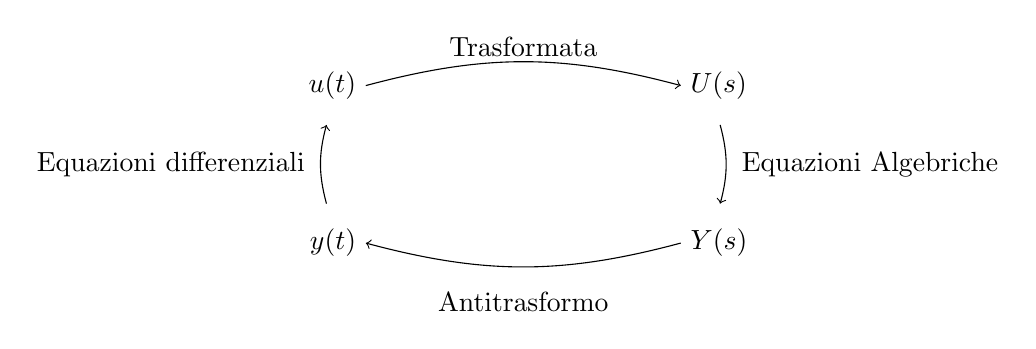
\begin{tikzpicture}
			\centering
			\draw[->] (-2,-1) node[left]{$ u(t) $} to[bend left = 15] (2,-1) node[right]{$ U(s) $};
			\draw (0,-0.75) node[above]{Trasformata};
			\draw[->] (2.5,-1.5) to[bend left = 15] (2.5, -2.5);
			\draw (2.65,-2) node[right]{Equazioni Algebriche};
			\draw[<-] (-2,-3) node[left]{$ y(t) $} to[bend right = 15] (2,-3) node[right]{$ Y(s) $};
			\draw (0,-3.5) node[below]{Antitrasformo}; 
			\draw[<-] (-2.5,-1.5) to[bend right = 15] (-2.5, -2.5);
			\draw (-2.65,-2) node[left]{Equazioni differenziali};
		\end{tikzpicture}
	\end{figure}
	\lablsubsection{Trasformata di Laplace}
	Sia $ f(t) $ funzione del tempo $ t\geq 0 $. Chiamo $ s $ la variabile complessa di \person{Laplace}. Si dice trasformata di \person{Laplace} di $ f(t) $ la funzione
	\begin{equation*}
		F(s) = \int_{0}^{\infty} f(t) e^{st}dt
	\end{equation*}
	La trasformata si indica anche come: 
	\begin{equation*}
		\mathcal{L}[f(t)]
	\end{equation*}
	\lablsubsection{Segnali Canonici}
	\subsubsection{Segnale a scalino}
	\begin{figure}[H]
		\begin{minipage}{.5\linewidth}
			\begin{tikzpicture}
				\assi{-1.5}{5}{$t$}{-0.5}{2}{$\text{sca}(t) $}
				\draw[color= darkorange,very thick] (-1.5,0) -- (0,0) -- (0,1) node[left]{$ 1 $} -- (5,1);
			\end{tikzpicture}
		\end{minipage}%
		\begin{minipage}{.5\linewidth}
			\[f(t) = \text{sca}(t) = \begin{cases}
				0 \,\, t<0\\
				1 \,\, t\geq0
			\end{cases}\]
		\end{minipage}
		\[\mathcal{L}[\text{sca}(t)] = \int_{0}^{\infty} 1\cdot e^{-st}dt = \left.-\frac{e^{st}}{s}\right|_{0}^{\infty} = \frac{1}{s}\]
	\end{figure}
	\subsubsection{Segnale ad impulso}
	Segnale di ampiezza infinita e durata infinitesima.
	\begin{equation*}
		\begin{cases}
			f(t) = \text{imp}(t) = 0 \space \forall t\not= 0\\
			\int_{-\infty}^{\infty} \text{imp}(t) = 1
		\end{cases}
	\end{equation*}
	Per trovare la trasformata uso un'approssimazione
	\begin{figure}[H]
		\begin{minipage}{.5\linewidth}
			\begin{tikzpicture}
				\assi{-1.5}{5}{$t$}{-0.5}{2}{$ \text{imp}(t) $}
				\draw[color= darkorange,very thick] (-1.5,0) -- (0,0) -- (0,1.5) node[left]{$\frac{1}{\varepsilon}$} -- (1,1.5) -- (1,0) node[below]{$\varepsilon$} -- (5,0);
			\end{tikzpicture}
		\end{minipage}%
		\begin{minipage}{.5\linewidth}
			\[f_\varepsilon = \begin{cases}
				\frac{1}{\varepsilon} \,\, 0\leq t\leq \varepsilon\\
				0 \,\, t>\varepsilon
			\end{cases}\]
		\end{minipage}
		\[\mathcal{L}[\text{imp}(t)] = \int_{0}^{\infty} \text{imp}(t)\cdot e^{-st}dt =\lim_{\varepsilon\to0}\int_{0}^{\infty}f_\varepsilon e^{-st}dt = 
		\lim_{\varepsilon\to0}\frac{1}{\varepsilon}\int_{0}^{\varepsilon}e^{-st}dt = \lim_{\varepsilon\to0} \left.-\frac{1}{\varepsilon}\frac{e^{-st}}{s}\right|_0^\varepsilon = \lim_{\varepsilon\to0} \frac{1-e^{\varepsilon s}}{\varepsilon s} = 1 \]
	\end{figure}
	\lablsubsection{Proprietà}
	\begin{itemize}
		\item Linearità
		\[\mathcal{L}\left[a_1f_1+a_2f_2\right] = a_1\mathcal{L}[f_1] + a_2\mathcal{L}[f_2]\]
		\item Traslazione nel dominio di 
		\[\mathcal{L}\left[e^{at}f(t)\right] = F(s-a)\]
		\item Traslazione nel dominio di t (ritardo)
		\[\mathcal{L}\left[f(t-\tau)\right] = e^{-s\tau}F(s) \space \tau>0\]
		\item Derivazione nel dominio di s
		\[\mathcal{L}\left[tf(t)\right] = -\frac{dF(s)}{ds}\]
		\item Derivazione nel dominio di t
		\[\mathcal{L}\left[\frac{df}{dt}\right] = sF(s) - f(0)\space \to \dot{x} = sX(s) -x(0)\]
	\end{itemize}
%%% Local Variables:
%%% mode: latex
%%% TeX-master: "master"
%%% End:

    \lecture{9}{lun 01 mag 2023 17:15}{Poli, zeri e G(s)}
	\lablsection{Poli e zeri}
	\lablsubsection{Definizione}
	\begin{itemize}
		\item Definisco \emph{poli} di $ F(s) $, i valori di s tali che $ F(s) = \infty $
		\item Definisco \emph{zeri} di $ F(s) $, i valori di s tali che $ F(s) = 0 $
		\item Se $ F(s) = \frac{N(s)}{D(s)} $, i \emph{poli} sono le radici di $ D(s) $ e gli \emph{zeri} sono le radici di $ N(s) $
	\end{itemize}
	\lablsubsection{Trasformate notevoli}
	\begin{figure}[H]
		\begin{minipage}{0.3\linewidth}
			\centering
			\begin{tikzpicture}
				\centering
				\assistd{2}{$ t $}{2}{$ \text{ram}(t) $}
				\draw[color=darkorange,thick] (0,0) -- (2,2);
			\end{tikzpicture}
			\begin{equation*}
				\text{ram}(t)=\begin{cases}
					0 \,\,\, t<0\\
					t \,\,\, t\geq0
				\end{cases}
			\end{equation*}
		\end{minipage}%
		\begin{minipage}{0.3\linewidth}
			\centering
			\begin{tikzpicture}{		
					\centering
					\assistd{2}{$ t $}{2}{$ \text{par} (t)$}}
				\draw[color=darkpurple,thick] (0,0.01) parabola[bend at start] (2,2);
			\end{tikzpicture}	
			\begin{equation*}
				\text{par}(t)=\begin{cases}
					0\,\,\, t<0\\
					\frac{t^2}{2}\,\,\, t\geq0
				\end{cases}
			\end{equation*}
		\end{minipage}
		\begin{minipage}{0.3\linewidth}
			{\tabulinesep = 1.2mm
				\begin{tabu}[H]{|c|c|}
					\hline
					$ f(t) $&$ F(s) $ \\
					\hline
					
					\Large imp(t) & $ 1 $\\\hline
					\Large sca(t) & \Large$ \frac{1}{s} $\\\hline
					\Large ram(t) & \Large$\frac{1}{s^2}$\\\hline
					\Large par(t) & \Large$ \frac{1}{s^3} $\\\hline
					\Large $ e^{at} $ & \Large$ \frac{1}{s-a} $\\\hline
					\Large $ \sin(\omega t) $ &\Large $\frac{\omega}{s^2 + \omega^2}$\\\hline
					\Large $ \cos(\omega t) $ &\Large $ \frac{s}{s^2 + \omega^2} $\\\hline
			\end{tabu}}
		\end{minipage}
	\end{figure}
	\lablsubsection{Antitrasformata}
	\lablsubsection{Teorema del valore iniziale (TVI)}
	Il \gls{tvi} recita come segue:\\
	Sia $\mathcal{L}\left[f(t)\right] = F(s) $, allora:\[f(0) = \lim_{s\to 0} sF(s) \]
	\lablsubsection{Teorema del valore finale (TVF)}
	Il \gls{tvf} recita come segue:\\
	Sia $\mathcal{L}\left[f(t)\right] = F(s) $ e $ F(s) $ razionale con tutti i poli a parte reale negativa o nulla, allora:
	\[\lim_{t\to\infty} f(t) = \lim_{s\to0}sF(s)\]
	\lablsubsection{Sviluppo di Heaviside}
	Vogliamo calcolare l'espressione analitica:
	\[F(s)=\frac{N(s)}{D(s)}=\frac{b_0 S^m+b_1 S^{m-1}+\ldots+b_m}{S^n+a_1 S^{n-1}+\ldots+a_n} \quad m \leq n\]
	Scrivo il denominatore come prodotto di fattori del tipo $ (s + p_i) $
	\begin{enumerate}
		\item Poli reali distinti
		\[D(s)=\left(s+p_1\right) \cdot\left(s+p_2\right) \ldots\left(s+p_n\right) \quad p_i \in \R \quad p_i \neq p_j \quad i=j\]
		Lo sviluppo di Heaviside
		\[F(s)=\frac{\alpha_1}{s+p_1}+\frac{\alpha_2}{s+p_2}+\ldots+\frac{\alpha_n}{s+p_n} \quad \alpha_i \text{ coeff. non noti}\]
		Per confronto tra il numeratore di $ F(s) $ e del suo sviluppo calcolo il minimo comune denominatore, trovo $ \alpha_i  $ e scrivo
		\[f(t)=\alpha_1 e^{-p_1 t}+\alpha_2 e^{-p_2 t}+\ldots+\alpha_n e^{-p_n t}\]
		\item Poli semplici reali e uno multiplo
		\[D(s)=\left(s+p_1\right)^k\left(s+p_2\right) \ldots\left(s+p_m\right) \quad p_i \in \R \quad p_i \neq p_j \quad i=j \quad m=n-(k-1)\]
		Lo sviluppo
		\[F(s)=\frac{\alpha_{1 k}}{\left(s+p_1\right)^k}+\frac{\alpha_{1 k-1}}{\left(s+p_1\right)^{k-1}}+\ldots+\frac{\alpha_{11}}{s+p_1}+\frac{\alpha_2}{\left(s+p_2\right)}+\cdots+\frac{\alpha_m}{s+p_m}\]
		I coefficienti si trovano come prima. L'espressione di $ f(t) $ è:
		\[f(t)=\alpha_{1 k} \frac{t^{k-1}}{(k-1) !} e^{-P_1 t}+\alpha_{1 k-1} \frac{t^{k-2}}{(k-2) !} e^{-P_1 t}+\ldots+\alpha_{11} e^{-P_1 t}+\ldots+\alpha_m e^{-P_m t}\]
		\item Poli reali semplici e una coppia di complessi coniugati
		\[\begin{gathered}
			D(s)=\left(s+p_1\right)\left(s+\bar{p}_1\right)\left(s+p_2\right) \cdots\left(s+p_m\right) \quad p_i \in \R \quad \begin{array}{l}
				p_i \neq p_j \quad i \neq \gamma \\
				m=n-1
			\end{array}
		\end{gathered}\]
		Scrivo $ P_1 = \sigma \pm \jmath \omega $. Sviluppo:
		\[F(s)=\frac{\beta s+\gamma}{s^2+2 \sigma s+\sigma^2+\omega^2}+\frac{\alpha_2}{s+p_2}+\ldots+\frac{\alpha_m}{s+p_m} \]
		I coefficienti si trovano come prima, $ f(t) $ è 
		\[f(t)=\beta e^{-\sigma t} \cos (\omega t)+\frac{\gamma^{-\beta \delta}}{\omega} e^{-\sigma t} \sin (\omega t)+\alpha_2 e^{-p_2 t}+\ldots+\alpha_m e^{-p_m t}\]
	\end{enumerate}
	\lablsubsection{Funzione di trasferimento (FdT) per sistemi LTI}
	\begin{equation*}
		\begin{cases}
			\dot{x} = Ax + Bu\\
			y = Cx+Du
		\end{cases}
		\quad x \in \R^n \, u\in\R^m \, y \in\R^P
	\end{equation*}
	Chiamo $ X(s), U(s), Y(s) $ le trasformate di $ x,u,y $. Applico $\mathcal{L} \left[\frac{df}{dt}\right]= sF(s) -x(0)$ 
	\[\begin{aligned}
		& \mathcal{L}[\dot{x}(t)]=s X(s)-x(0) \\
		& \mathcal{L}[A x]=\left(\begin{array}{l}
			\mathcal{L}\left[a_{11} x_1+\ldots+a_{1 n} x_n\right] \\
			\mathcal{L}\left[a_{n 1} x_1+\ldots+a_{n n} x_n\right]
		\end{array}\right)=\left(\begin{array}{cc}
			a_{11} X_1(s) \ldots a_{1 n} X_n(s) \\
			a_{n 1} X_1(s) \ldots a_{n n} X_n(s)
		\end{array}\right)=A X(s)
	\end{aligned}\]
	Procedendo in modo analogo con $ B,C ,D $ trovo un \underline{sistema algebrico}.
	\[\begin{aligned}
		&sX(s) - x(0) = AX(s) + BU(s)\\
		&Y(s) = CX(s) + DU(S)
	\end{aligned}\]
	Ponendo $ x(0)  = 0$ trovo la FdT
	\[\begin{aligned}
		&Y(s)= G(s)U(s)\\
		&G(s) = C(sI-A)^-1B+D
	\end{aligned}\]
	Vale per i sistemi MIMO e SISO. Per i sistemi SISO posso scrivere
	\[G(s) = \frac{N(s)}{D(s)}\]
	\lablsection{G(s)}
	Date A, B, C, D allora la FdT si trova come:
	\[G(s) = C(sI-A)^-1B+D\]
	Scrivo la trasformata di \person{Laplace} e le proprietà sostituendo $ \dot{x} = sX(s) $ e condizioni iniziali nulle. Trovo un sistema algebrico e lo risolvo trovando la relazione tra $ Y(s) $ e $ U(s) $
	\lablsubsection{Struttura di G(s) (SISO)}
	\[\begin{aligned}
		&G(s) = C(sI-A)^-1B + D\\
		&(sI-A)^-1 = \frac{1}{det(sI-A)} \left[\begin{array}{ccc}
			k_{11}(s) & \ldots & k_{1 n}(s) \\
			\vdots & \ddots & \vdots \\
			k_{n 1}(s) & \ldots & k_{n n}(s)
		\end{array}\right]
	\end{aligned}\]
	\begin{itemize}
		\item I complementi algebrici $ x_{ij} $ sono polinomi di grado non superiore a $ n-1 $
		\item Il determinante di $ (sI -A ) $ è il polinomio caratteristico di grado $ n $
		\item $ C(sI-A)^-1B $ da luogo a una combinazione lineare dei complementi algebrici $ k_{ij} $
		\item Sommando $ D $ potrei avere un numero di grado $ n $, ma il denominatore è sempre di grado $ n $. In ogni caso ho una funzione razionale:
		\[G(S) = \frac{N(s)}{D(s)} = \frac{Y(s)}{U(s)}\]
	\end{itemize}
	\nota{il grado del numeratore non può essere superiore a quello del denominatore, non posso avere più zeri che poli.}
	I poli, cioè le radici di $ D(s) $, cioè ci $ \det(sI-A) $ coincidono eventualmente con gli autovalori di A. Questo è vero solo se non ho cancellazioni tra le radici del numeratore e le radici del denominatore.
	\subsubsection{Proprietà di invarianza di G(s)}
	La FdT è una proprietà strutturale. Dimostrazione:
	\\Sia$ \quad \hat{A}=T A T^{-1}, \hat{B}=T B, \hat{C}=C T^{-1}, \hat{D}=D$
	\[
	\begin{aligned}
		& T: \operatorname{det}(T) \neq 0 \\
		& \hat{G}(s)=\hat{C}(s I-\hat{A})^{-1} \hat{B}+\hat{D}
	\end{aligned}
	\]
	Voglio dimostrare che $\hat{G}(s)=\hat{C}(s I-\hat{A})^{-1} \hat{B}+\hat{D}=G(s) \quad$ (considerando $I=TT^{-1}$ )
	\[
	\begin{aligned}
		\hat{G} & =\hat{C}(s I-\hat{A})^{-1} \hat{B}+D=C T^{-1}(\underbrace{s T T^{-1}-T A T^{-1}}_{T s T^{-1}-T A T^{-1}}) T B+D= \\
		& =C T^{-1}(T(\underbrace{s I-A}_B) T^{-1})^{-1} T B+D=C T^{-1} T(s I-A)^{-1} I^{-1} T B+D= \\
		& =C(s I-A)^{-1} B+D=G(s) 
	\end{aligned}
	\]
	\subsubsection{Cancellazione e dinamiche nascoste}
	Noto che $ G(s) $ è una rappresentazione esterna del sistema ho cancellazione quando il numero di poli di $ G(s) $ è $ D<n $ dove $ n $ è il numero di autovalori di A. Se ho cancellazioni ho una dinamica nascosta, legata alle definizioni di raggiungibilità e osservabilità.
	\lablsubsection{Raggiungibilità}
	%\begin{figure}[H]
	%	\begin{minipage}{.5\linewidth}
		%		\begin{tikzpicture}[x=5mm,y=5mm,decoration={mark random y steps,segment length=3mm,amplitude=1mm}]
			%			\assistd{3}{$ u $}{3}{$ t $}
			%			\path[decorate]   (0,2) -- (3,2);
			%			 \draw[blue,thick] plot[variable=\x,samples at={1,...,\arabic{randymark}},smooth] (randymark\x);
			%			 \draw (1.5,2) node[above]{$ \tilde(u) $}
			%			 \draw (3,0) --- (3,2)
			%		\end{tikzpicture}
		%	\end{minipage}
	%\end{figure}
	\begin{figure}[H]
		\centering
		\includegraphics[width=0.7\linewidth]{Images/RaggiungibilitàIPE.png}
	\end{figure}
	Uno stato $\tilde{x}$ di un sistema LTI si dice raggiungibile se esiste un tempo finito $ 0\leq t \leq \tilde{t} $ e un ingresso $ \tilde{u}(t) $ definito in $ 0\leq t \leq \tilde{t} $, tale che, detto $ \tilde{x}_{f}(t) $ il moto forzato corrispondente, si ha che $ \tilde{x}_{f}(\tilde{t}) = \tilde{x}$
	\subsubsection{Test di raggiungibilità}
	Calcolo la matrice di raggiungibilità 
	\[K_R=\left(\begin{array}{lllll}
		B & A B & A^2 B & \ldots & A^{n-1} B
	\end{array}\right)\]
	Il sistema si dice completamente raggiungibile se $ \operatorname{rank}(K_R) = n $
	\lablsubsection{Osservabilità}
	\begin{figure}[H]
		\centering
		\includegraphics[width=0.7\linewidth]{Images/Osservabilità}
	\end{figure}
	Uno stato $ \tilde{x} $ di un sistema LTI si dice non osservabile se $\forall \tilde{t}>0$ finito, detto $ \tilde{y}_\mathcal{l}(t)$ moto libero dell'uscita generato da $\tilde{x}$ ho che $ \tilde{y}_\mathcal{l}(t)=0 $ $ 0\leq t\leq\tilde{t} $
	\subsubsection{Test di osservabilità}
	Calcolo la matrice di osservabilità 
	\[K_O=\left(\begin{array}{lllll}
		C^T & A^TC^T & A^{T^2} C^T & \ldots & A^{T^{n-1}} C^T
	\end{array}\right)\]
	Il sistema si dice completamente osservabile se $ \operatorname{rank}(K_O) = n $\\
	\\
	\nota{la raggiungibilità e l'osservabilità di un sistema sono proprietà strutturali.} 
%%% Local Variables:
%%% mode: latex
%%% TeX-master: "maste"
%%% End:

    \lecture{10}{lun 01 mag 2023 17:16}{Realizzazione e forme di G(s)}
	\lablsection{Realizzazione}
	\[\left(A,B,C,D\right)\to G(s)\]
	Ora vogliamo scrivere una realizzazione in spazio di stato a partire dalla $ G(s) $. Notiamo un paio di cose
	\begin{itemize}
		\item Questo problema ammette infinite soluzioni.
		\item Le realizzazioni in cui A ha dimensioni uguali al grado del denominatore di $ G(s) $ su dicono \emph{minime}.
		\item Le realizzazioni minime sono completamente raggiungibili e osservabili.
	\end{itemize}
	\lablsubsection{Forme canoniche}
	\[G(s) = \frac{N(s)}{D(s)}\quad \operatorname{grad}(D(s)) = n  \text{ se } \operatorname{grad}(N(s))= n \to \text{ \emph{Sistema Proprio} }\]
	Scrivo per comodità
	\[\begin{aligned}
		& G(s)=\frac{\tilde{N}(s)}{D(s)}+b_n \quad \operatorname{grad}(\tilde{N}(s))=n-1 \\
		& G(s)=\frac{b_{n-1} s^{n-1}+b_{n-2} s^{n-2}+\ldots+b_1 s+b_0}{s^n+a_{n-1} s^{n-1}+a_{n-2} s^{n-2}+\ldots+a_1 s+a_0}
	\end{aligned}\]
	\subsubsection{La forma canonica di raggiungibilità (o controllo)}
	\[A=\left(\begin{array}{cccc}
		0 & 1 & &0 \\
		\vdots&\ddots  &\ddots&  \\
		0& &  0& 1 \\
		-a_0&-a_1 & \cdots & a_{n-1}
	\end{array}\right) \quad B=\left(\begin{array}{c}
		0 \\
		0 \\
		\dots\\
		0 \\
		1
	\end{array}\right) \quad c=\left(\begin{array}{llll}
		b_0 & b_1 & \ldots & b_{n-1}
	\end{array}\right) \quad D=b_n\]
	Osservazione: Le forme canoniche godono delle proprietà di osservabilità e raggiungibilità.
	\lablsection{Parametri caratteristici di G(s)}
	\lablsubsection{Forma in costante di trasformata, Poli e Zeri (EVANS)}
	\begin{figure}[H]
		\begin{minipage}{.5\linewidth}
			\[G(s)=\frac{\rho \prodc_i\left(s+z_i\right)}{s^g \prodc_k\left(s+p_k\right)}\]
		\end{minipage}
		\begin{minipage}{.5\linewidth}
			\[\rho \to \text{Costante di trasferimento o EVANS} \quad z_i\to \text{Zeri}\quad p_k \to poli\]
			\[g\to\text{tipo}\begin{cases}
				g>0 \quad \# \text{ poli nell'origine}\\
				g = 0\quad \text{non ho poli o zeri nell'origine}\\
				g<0 \quad \# \text{ zeri nell'origine}
			\end{cases}\]
		\end{minipage}
	\end{figure}
	Se ho poli e zeri complessi coniugati li estraggo così:
	\[s^2 + 2\xi\omega_ns + \omega_n^2\quad \omega_n >0\]
	Le cui radici sono:
	\begin{figure}[H]
		\begin{minipage}{.5\linewidth}
			\centering
			\[s_{1,2} = - \xi\omega_n\pm\xi\omega\sqrt{1-\xi^2},\quad \left|\xi\right|\]
			\begin{tikzpicture}[ultra thick]
				\draw[->,thin] (-3,0) -- (2,0) node[below]{};
				\draw[->,thin] (0,-3) -- (0,3) node[left]{};
				\draw (0,0) node[above right]{$ 0 $};
				\draw[dashed,color=red] (-2,-3) -- (-2,3);
				\draw[dotted,color=blue] (0,0) -- (-2, 2);
				\draw[dotted,color=blue] (0,0) -- (-2, -2);
				\draw[dash dot dot,color=darkorange] (-1.5,0) arc[start angle=180,end angle=135,radius=1.5];
				\draw (-1.5,0) node[above left]{$\mathcolor{darkorange}{ \alpha }$};
				\draw[color=darkorange] (0,0) node[below right]{$ \xi= \cos\alpha $};
			\end{tikzpicture}
		\end{minipage}
		\begin{minipage}{.5\linewidth}
			\[
			\begin{aligned}
				\omega_n&\to\text{Pulsazione naturale, distanza dall'origine}\\
				\xi &\to \text{Smorzamento, rappresenta il coseno dell'angolo con il semiasse negativo}\\
				\xi < 0 &\to\text{Radici a destra}
			\end{aligned}
			\]
		\end{minipage}
	\end{figure}
	Riscrivendo $ G(s) $
	\[\begin{gathered}
		G(s)=\frac{\rho}{s^g} \frac{\prodc_i\left(s+z_i\right) \prodc_i\left(s^2+2\xi_{z_i} \omega_{z_in} s+\omega_{z_in}^2\right)}{\prodc_k\left(s+p_k\right) \prodc_k\left(s^2+2 \xi_{p_k} \omega_{p_k} s+\omega_{p_{k n}}^2\right)} \\\\ \mid \xi_{z_i}|,| \xi_{p_k} \mid<1 \text{ e }w_{z_i n}, w_{p_k n}>0 
	\end{gathered}\]
	\lablsubsection{Forma in guadagno, costanti di tempo}
	
	\twomini{\[G(s)=\frac{\mu}{s^g} \frac{\prodc_i\left(1+s \tau_i\right)}{\prodc_k\left(1+s T_k\right)}\]}{\[\mu \to \text{Guadagno di $ G(s) $}\]
		\[\tau_i\to \text{Costanti di tempo degli zeri}\]
		\[T_i\to \text{Costanti di tempo dei poli}\]}
	
	Posso estrarre i poli complessi coniugati
	\[
	G(s)=\frac{\frac{\mu}{s^g} \prodc_i\left(1+\tau_i\right) \prodc_i\left(1+\frac{2 \xi_{z_i} s}{\omega_{z_i}^2}+\frac{s^2}{\omega_{2 i n}^2}\right)}{\prodc_k\left(1+T_k s\right) \frac{\pi}{k}\left(1+\frac{2 \xi_{P_k} s}{\omega_{p_{k n}}}+\frac{s^2}{\omega_{p_{k n}}^2}\right)}
	\]
%%% Local Variables:
%%% mode: latex
%%% TeX-master: "master"
%%% End:

    \lecture{11}{lun 01 mag 2023 17:17}{Guadagno e costante di tempo, sistemi del primo ordine}
	\lablsection{Guadagno e costante di tempo}
	\twomini{\[G(s) = \frac{\mu}{s^g}\frac{\prodc_i(1+s\tau_i)}{\prodc_k(1+sT_k)}\]}{\[
		\begin{aligned}
			\text{Zeri}&:-\frac{1}{\tau_i}\\
			\text{Poli}&: -\frac{1}{T_k}
		\end{aligned}
		\]}
	Per quanto riguarda il guadagno $ \mu $ valuto due sotto casi
	\begin{enumerate}
		\item \emph{Guadagno statico}\\$ g=0 \to \mu = \lim_{s\to0}G(s) \approx G(o)$
		\\Capiamo di cosa si tratta:
		\twomini{\[\begin{cases}
				\dot{x} = Ax+Bu\\
				y = Cx+Du
			\end{cases}\]}{\[G(s)=C(sI-A)^-1B+D\]}
		Valuto il sistema all'equilibrio dato $ u = \overline{u}\,\, t\geq0 $
		\begin{equation*}
			\begin{cases}
				\overline{x} = -A^{-1} B\overline{u}\\
				\overline{y} = -CA^{-1}\overline{u} + D\overline{u} =\left( -CA^{-1} + D\overline{u}\right)
			\end{cases}
		\end{equation*}
		Scrivo $ G(0) = -CA^{-1}B + D $, quindi $ \mu = \frac{\overline{y}}{\overline{u}} $ e cioè il guadagno statico è il rapporto tra uscita ed ingresso all'equilibrio.
		\item \emph{Guadagno semplice o generalizzato} $ g\neq 0 \to \mu = \lim_{s\to0} s^gG(s)$
	\end{enumerate}
	\lablsubsection{Risposte Canoniche}
	I parametri (o indici) caratteristici della risposta allo scalino: vedremo funzioni del primo o del secondo ordine.
	\nota{Valuteremo il moto forzato. La stabilità del sistema non dipende dagli ingressi}
	Disegniamo un generico segnale:
	\begin{figure}[H]
		\centering
		\includegraphics[width=0.7\linewidth]{Images/generico_segnale}
	\end{figure}
	Nel quale:
	\begin{itemize}
		\item $ T_s $: tempo di salita: è il tempo che il segnale impiega per passare da $ 0.1y_{\infty} $ a $ 0.9y_{\infty} $, con $ y_{\infty} $ il valore del segnale a transitorio esaurito.
		\item $ T_{a_{\epsilon}} $: tempo di assestamento al $ (100\pm\epsilon)\% $ di $ y_\infty $, è il tempo impiegato dal segnale per entrare nella striscia $ \pm\epsilon\% $ di $ y_\infty $.
		\item $ S $: massima sovra elongazione.
		\item $ S_\% =\frac{ \displaystyle\max_\tau \left[ y (\tau)\right] - y_\infty }{ y_\infty }$ massima sovra elongazione percentuale. 
	\end{itemize}
	\lablsection{Sistemi del primo ordine}
	\begin{enumerate}
		\item $ G(s) $ strettamente propria (cioè grado del denominatore è 1 mentre del numeratore è 0)
		\begin{enumerate}
			\item[\textbf{a.}] $ g=0 \to G(s) = \frac{\mu}{sT+1}$, polo: $ \frac{-1}{T} $
			$ G(s) $ è A.S. quando $ T>0 $.
			\begin{itemize}
				\item Risposta allo scalino ($ u(t) = \operatorname{sca}(t) \to U(s) = \frac{1}{s} $)
				\begin{equation*}
					Y(s) = G(s) \frac{1}{s} = \frac{\mu}{s(sT+1)}
				\end{equation*}
				Antitrasformo e trovo
				\begin{equation*}
					y(t) = \mu (1-\exp^{-t/T}) \quad t\geq0 \qquad \dot{y}(0) =\frac{\mu}{T}
				\end{equation*}
				\twomini{
					\begin{figure}[H]
						\centering
						\includegraphics[width=0.7\linewidth]{Images/risp_scalino1}
				\end{figure}}{Più T è piccolo, più veloce sarà la risposta}
				Sto assumendo per semplicità $ \mu>0 $ ma è anche possibile che $\mu$ sia negativo. In questo caso il grafico si specchia sull'asse delle ascisse.\\\\
				Usando il \emph{TVF} (\cref*{subsec:Teorema del valore finale (TVF)}) con (T>0) trovo:
				\begin{equation*}
					\displaystyle\lim_{t\to\infty} y(t) = \lim_{s\to0} sY(s) = \mu
				\end{equation*}
				A transitorio esaurito ho un valore pari a $\mu$. Il tempo di assestamento è pari a 
				\begin{equation*}
					T_{a\epsilon} =4.6T 
				\end{equation*}
				\item\emph{risposta all'impulso}
				\begin{equation*}
					u(t) =\operatorname{imp}(t) \to U(s)
					Y(s) = G(s) \cdot 1=\frac{\mu}{sT +1}
				\end{equation*}
				Antitrasformo e trovo
				\begin{equation*}
					y(t) = \frac{\mu}{T}\exp^{-t/T} \quad t\geq 0
				\end{equation*}
				\nota{La risposta all'impulso è la derivata della risposta allo scalino}
				\begin{center}
					\begin{tikzpicture}
						\begin{axis}[
							axis lines = left,
							xlabel = $t$,
							ylabel = $y$,
							no markers,
							xticklabel = \empty,
							yticklabel = \empty]
							\addplot+ [smooth,decorate,red]{e^-x};
							\addlegendentry{$T>0\, G(s)$ A.S.}
						\end{axis}
					\end{tikzpicture}
				\end{center}
				\item \emph{$g = 1$ $G(s) = \frac{\mu}{s}$}
				\item \emph{Risposta allo scalino}\\
				$Y(s) = G(s) \cdot \frac{1}{s} = \frac{\mu}{s^2}$
				Antitrasformo $y(t) = \mu \cdot\operatorname{ram}(t)$\\
				\begin{center}
					\begin{tikzpicture}
						\begin{axis}[
							axis lines = left,
							xlabel = $t$,
							ylabel = $y$,
							no markers,
							xticklabel = \empty,
							yticklabel = \empty]
							\addplot{x};
						\end{axis}
					\end{tikzpicture}
				\end{center}
				\item \emph{Risposta all'impulso}\\
				$Y(s) = G(s) \cdot 1 = \frac{\mu}{s}$\\
				La risposta è uno scalino di ampiezza $\mu$.\\
				$y(t) = \mu\operatorname{sca}(t)$\\
				\begin{center}
					\begin{tikzpicture}
						\begin{axis}[axis lines = left,
							xlabel = $t$,
							ylabel = $y$,
							no markers,
							xticklabel = \empty,
							yticklabel = \empty]
						\end{axis}
					\end{tikzpicture}
				\end{center}
			\end{itemize}
			\item $G(s)$ proprie $\operatorname{grad}(D(s))=\operatorname{grad}(N(s))=1$
			  \subitem $g=0$ $G(s) = \mu \\frac{1+st}{1+sT}$
			  Antitrasformo
			  \[y(t) = \mu (1 +(\frac{t}{T}-1)\exp^{\\frac{-t}{T}}) \quad t\geq0\]
			  Assumo $\mu>0 , T>0 $ (\gls{as})\\
			  Ora non resta che da capire cosa succede al variare di $t$.
			  % TODO: add graphs
			  Osservazioni:\\
			  \begin{itemize}
				\item La risposta all'impulso è la derivata della risposta allo scalino: $y(t) = \frac{\mu}{T}(\frac{t}{T}-1)\exp^{\frac{-t}{T}}$
				\item Nei primi due casi con $t>0$, la risposta \textit{anticipa}, quella del caso senza zero.
				\item Quando $t<0$ il sistema si dice a fase non minima
			  \end{itemize}
			  \item $g=1$ $G(s) = \mu \frac{st+1}{s}$
				\subitem Risposta allo scalino
				\[Y(s) = G(s) \cdot \frac{1}{s} = \frac{\mu}{s^2}(st+1)\]
				Antitrasformo
				\[y(s) = \mu t +\mu \operatorname{ram}(t)\quad t\geq0\]
				Assumo $\mu>0$
				%% TODO: add graphs
				\item $g=-1$ $G(s) = \mu \frac{s}{1+st}$
				  \subitem Risposta allo scalino
				  \[Y(s) = G(s)\frac{\mu}{st+1}\]
				  Noto che è uguale alla risposta all'impulso di una $G(s)$ strettamente propria con $g=0$
				 % TODO: copy graph from file
		\end{enumerate}
	\end{enumerate}
	\lablsubsection{Sistemi del secondo ordine}
	\begin{enumerate}
	  \item Poli reali e nessuno zero
		\twomini{\[G(s) = \frac{\mu}{(1+sT_1)(1+sT_2)}\]}{Poli: $- \frac{1}{T_1} $ , $- \frac{1}{T_2}$ \\\gls{as} $T_1,T_2 >0$}
		\subitem Risposta allo scalino
		\[Y(s) = G(s) \cdot \frac{1}{s} = \frac{\mu}{s(1+sT_1)(1+T_2) \quad \mu>0}\]
		Applico i teoremi \gls{tvi} e \gls{tvf}
		\[y(0) = \liminf_{s \to \infty} sY(s) = 0\]
		\[\dot{y}(0) = \liminf_{s \to \infty} s\underbrace{(sY(s) - y(0))}_{\L[\dot{y(t)}]} = 0 \]
		\[\ddot{y}(0) = \liminf_{s \to \infty} s\underbrace{(s^2Y(s) - \dot y(0))}_{\L[\ddot{y}(t)]} = \frac{\mu}{T_1 T_2}>0 \]
		\[y(\infty) = \limsup_{s \to 0} sY(s) = \mu\]
		Applico Heaviside
		\[y(t) = \mu \left[1 - \frac{T_1}{T_1 - T_2} \exp^{\frac{-t}{T_1}}+\frac{T_2}{T_1 - T_2} \exp^{\frac{-t}{T_1}}\right] \quad t\geq 0\]
		% Todo: inserisci grafico
		Noto che $T_1 \simeq T_2 $ vuol dire che i poli si influenzano reciprocamente, se una delle due $T$ è più grande, allora
		domina sull'altra e posso approssimare la $G(s)$ come una funzione del primo ordine.
		\begin{equation*}
		 T_1 >> T_2 \to y(t) \simeq \mu (1- \exp^{\frac{-t}{T_1}})
		\end{equation*}
		Analogalmente per $T_2 >> T_1$. Il tempo di assestamento sarà circa $4,6 T_i \quad T_i>>T_j$.\\
		Nota: se $T_1 =T_2 =T$, il tempo di assestamento è $T_{a1} = 6,664T$
		\item Poli reali e uno zero
		  \[G(s) = \mu \frac{(1+st)}{(1+sT_1)(1+sT_2)}\quad \begin{aligned}
			\mu >0\\
			T_1,T_2 >0
		  \end{aligned} \]
		  \subitem Risposta allo scalino
		  \[Y(s) = G(s) \frac{1}{s} = \frac{\mu}{s}\frac{(1+st)}{(1+sT_1)(1+sT_2)}\]
		  Applico \gls{tvi} e \gls{tvf} e trovo
		  \[y(0) = 0 \quad,\quad \dot y(0) = \frac{\mu t}{T_1T_2}\quad,\quad y(\infty) = \mu\]
		  %TODO: inserisci grafici
		  \item Poli complessi coniugati
		\begin{equation*}
			G(s) = \mu \frac{\omega_n^2}{s^2 +2\xi\omega_ns +\omega_n^2}
			\qquad\qquad 
			\begin{aligned}
				&\mu >0\\
				&\omega_n: \text{Pulsazione naturale}\\
				&\xi: \text{Smorzamento}
			\end{aligned}
		\end{equation*}
			\subitem Risposta allo scalino
			\[y(0) = 0 \quad,\quad \dot y(0) = \frac{\mu t}{T_1T_2}\quad,\quad \ddot y(0)=\mu\omega_n^1>0\\y(\infty) = \mu\]
			Antitrasformo
			\[y(t)=\mu\left[1- \frac{1}{\sqrt{1-\xi^2}}\exp^{-\xi\omega_nt}\sin(\omega_n\sqrt{1-\xi^2}t+\alpha)\right]\quad t\geq0\]
			Con $\xi = \cos(\alpha)$\\
			Noto che $\xi=0$ significa che ci sono due poli coniugati a parte reale nulla.
			\[y(t) = \mu [1-\cos(\omega_nt)]\]
			\begin{tikzpicture}
			  \begin{axis}[
			  	axis lines = middle,
			  	xlabel = $t$,
			  	ylabel = $y$,
			  	no markers,
			  	xticklabel = \empty,
			  	yticklabel = \empty,
			  	xmin=0,
			  	xmax= 4*pi,
			  	ymax=1.1]
				\addplot[red,domain=0:4*pi,samples=200]{cos(deg(x))};
			  \end{axis}
			\end{tikzpicture}\\
			Considero ora $\xi > 0 $: La risposta è compresa tra due funzioni esponenziali:\\
			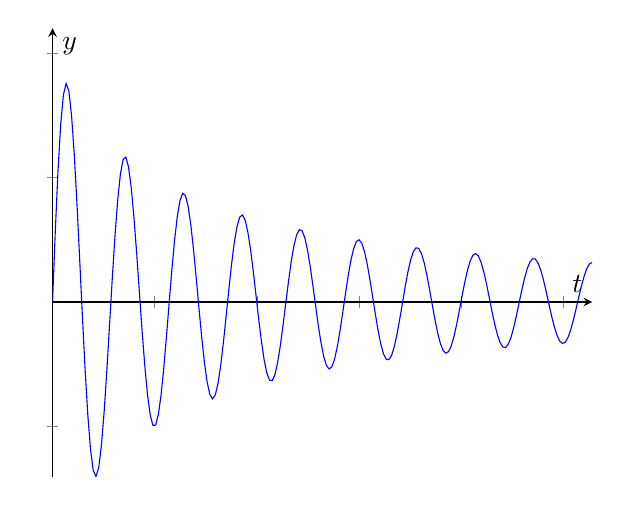
\begin{tikzpicture}
			  \begin{axis}[
			  	axis lines = middle,
			  	xlabel = $t$,
			  	ylabel = $y$,
			  	no markers,
			  	xticklabel = \empty,
			  	yticklabel = \empty,
			  	xmin=1,
			  	xmax= 2*pi,
			  	ymax=1.1]
				\addplot[blue,domain=1:2*pi,samples=200]{1/x * cos(deg(x)*11)};
				%todo: errore in questo grafico
			  \end{axis}
			\end{tikzpicture}\\
			Sovra-elongazione massima percentuale: $S_\%=100\cdot \exp^{(\frac{-\xi\pi}{\sqrt{1-\xi^2}})} $
			Le sovra-elongazione dipendono da $\xi$: più alto è $\xi$ maggiore è lo smorzamento
			%todo: aggiugi grafico
			Troviamo il tempo di assestamento $(\varepsilon=1)$ prendo un inviluppo esponenziale
			\[\mu (1-\exp^{-\xi\omega_nT_{a1}})=0.99\mu \to \xi \omega_nT_{a1} = h 100\]
			\[T_{a1} = \frac{\ln(100)}{\xi\omega_n}\simeq \frac{4.6}{\xi\omega_n}\]
	\end{enumerate}
%%% Local Variables:
%%% mode: latex
%%% TeX-master: "master"
%%% End:

    % end lectures
\end{document}
%%% Local Variables:
%%% mode: latex
%%% TeX-master: t
%%% End:
